\documentclass{article}


% if you need to pass options to natbib, use, e.g.:
    \PassOptionsToPackage{numbers, compress}{natbib}
% before loading neurips_2022

% ready for submission

% to compile a preprint version, e.g., for submission to arXiv, add add the
% [preprint] option:
% \usepackage[preprint]{neurips_2023}
\usepackage[final]{neurips_2023}

% to compile a camera-ready version, add the [final] option, e.g.:
%     \usepackage[final]{neurips_2023}


% to avoid loading the natbib package, add option nonatbib:
% \usepackage[nonatbib]{neurips_2023}

\usepackage[utf8]{inputenc} % allow utf-8 input
\usepackage[T1]{fontenc}    % use 8-bit T1 fonts
\usepackage{hyperref}       % hyperlinks
\usepackage{url}            % simple URL typesetting
\usepackage{booktabs}       % professional-quality tables
\usepackage{amsfonts}       % blackboard math symbols
\usepackage{nicefrac}       % compact symbols for 1/2, etc.
\usepackage{microtype}      % microtypography
\usepackage{xcolor}         % colors
\usepackage{graphicx}
\usepackage{comment}
\usepackage{authblk}
\usepackage{amsmath}
\usepackage{wrapfig}
\usepackage{booktabs}
\usepackage[rightcaption]{sidecap}
\hyphenpenalty=9999

\definecolor{VGG-19}{RGB}{174, 199, 232}
\definecolor{Inception-V3}{RGB}{34,120,181}
\definecolor{ResNet-50}{RGB}{47, 161, 72}
\definecolor{ViT-B}{RGB}{127, 127, 127}
\definecolor{Swin-B}{RGB}{158, 208, 138}
\definecolor{MLPMixer-B}{RGB}{214, 42, 40}
\definecolor{CORnet-S}{RGB}{247, 182, 209}
\definecolor{Harmonization}{RGB}{197, 177, 214}
\definecolor{ECOSET}{RGB}{199, 199, 199}
\definecolor{SimCLR}{RGB}{146, 104, 173}
\definecolor{MoCo-v3}{RGB}{196, 157, 149}
\definecolor{DINO}{RGB}{141, 87, 76}
\definecolor{MAE}{RGB}{216, 122, 178}
\definecolor{CLIP}{RGB}{245, 127, 32}
\definecolor{IPCL}{RGB}{188, 190, 50}
\definecolor{Noisy Student}{RGB}{246, 151, 151}
\definecolor{SWSL}{RGB}{252, 187, 120}

\definecolor{Blue}{RGB}{50,50,200}
\newcommand{\edited}[1]{\textcolor{Blue}{#1}}
\definecolor{Orange}{RGB}{255,127,80}
\newcommand{\kushin}[1]{\textcolor{Orange}{#1}}

\title{SEVA: Leveraging sketches to evaluate alignment between human and machine visual abstraction}

% Leveraging sketches to evaluate visual abstraction in humans and machines


% The \author macro works with any number of authors. There are two commands
% used to separate the names and addresses of multiple authors: \And and \AND.
%
% Using \And between authors leaves it to LaTeX to determine where to break the
% lines. Using \AND forces a line break at that point. So, if LaTeX puts 3 of 4
% authors names on the first line, and the last on the second line, try using
% \AND instead of \And before the third author name.

\author[ ]{Kushin Mukherjee$^{1}$\footnote[1]{}}
\author[ ]{Holly Huey$^{2}$\footnote[1]{}}
\author[ ]{Xuanchen Lu$^{2}$\footnote[1]{}}
\author[ ]{Yael Vinker$^{3}$\footnote[1]{}}
\author[ ]{Rio Aguina-Kang$^{2}$}
\author[ ]{Ariel Shamir$^{4}$}
\author[ ]{Judith E. Fan$^{2,5}$}


\affil[ ]{University of Wisconsin-Madison$^1$}
\affil[ ]{University of California, San Diego$^2$}
\affil[ ]{Tel-Aviv University$^3$}
\affil[ ]{Reichman University$^4$}
\affil[ ]{Stanford University$^5$}


\begin{document}

\footnotetext[1]{$^{/*}$Equal contribution}


\maketitle


\begin{abstract}
  % The abstract paragraph should be indented \nicefrac{1}{2}~inch (3~picas) on
  % both the left- and right-hand margins. Use 10~point type, with a vertical
  % spacing (leading) of 11~points.  The word \textbf{Abstract} must be centered,
  % bold, and in point size 12. Two line spaces precede the abstract. The abstract
  % must be limited to one paragraph.

Sketching is a powerful tool for creating abstract images that are sparse but meaningful. Sketch understanding poses fundamental challenges for general-purpose vision algorithms because it requires robustness to the sparsity of sketches relative to natural visual inputs and because it demands tolerance for semantic ambiguity, as sketches can reliably evoke multiple meanings. While current vision algorithms have achieved high performance on a variety of visual tasks, it remains unclear to what extent they understand sketches in a human-like way. Here we introduce \texttt{SEVA}, a new benchmark dataset containing approximately 90K human-generated sketches of 128 object concepts produced under different time constraints, and thus systematically varying in sparsity. We evaluated a suite of state-of-the-art vision algorithms on their ability to correctly identify the target concept depicted in these sketches and to generate responses that are strongly aligned with human response patterns on the same sketch recognition task. We found that vision algorithms that better predicted human sketch recognition performance also better approximated human uncertainty about sketch meaning, but there remains a sizable gap between model and human response patterns. To explore the potential of models that emulate human visual abstraction in generative tasks, we conducted further evaluations of a recently developed sketch generation algorithm \cite{vinker2022clipasso} capable of generating sketches that vary in sparsity. We hope that public release of this dataset and evaluation protocol will catalyze progress towards algorithms with enhanced capacities for human-like visual abstraction.
\end{abstract}


% We conduct further evaluations of a recently developed algorithm \cite{vinker2022clipasso} capable of generating sketches that vary in sparsity to explore to what degree these sketches manifest signatures of human-generated sketches.

\section{Introduction}

%% Visual abstraction is key challenge for AI
%% Sketch generation and understanding as key case study in visual abstraction 
% \subsection{Sketches as paradigmatic case study in visual abstraction}

Abstraction is key to how humans understand the external world. 
Abstraction enables distillation of individual sensory experiences into compact latent representations that support learning of new concepts \cite{smith2002object, kemp2007learning, murphy2004big, goldstone2013concepts} and efficient communication about these concepts with others \cite{fan2020pragmatic, tessler2019language, hawkins2023visual, gentner2017analogy}.
For example, while no two roses are identical, people can rapidly infer what properties make a flower a \textit{rose} and not some other kind of flower from just a few examples \cite{xu2007word, lake2020people}, especially when these examples are selected to support such strong inferences \cite{gweon2010infants, shafto2014rational}.

\subsection{Human Visual Abstraction as Key Target for AI}
\textit{Visual abstraction} enables humans to express what they know about the visual world by creating external representations that highlight the information they judge to be most relevant in any given context---for instance, pictures that highlight the visual features that are diagnostic of a \textit{rose} in a botanical field guide \cite{fan2018common, fan2020pragmatic, viola2017pondering}. 
Critically, there are many different ways to depict even the same object---from a detailed illustration to a simple sketch. 
The Spanish artist Pablo Picasso famously demonstrated this point in \textit{The Bull} (1945), a series of 11 lithographs of bulls, each sparser than the last (Fig.~\ref{fig:bulls}).
While some of the drawings in this series look more realistic and others more stylized, all of these images remain evocative of a \textit{bull} (and perhaps other similar animals, such as a \textit{moose} or \textit{buffalo}) to most human viewers.

\begin{wrapfigure}{r}{0.35\textwidth}
    \centering
    \includegraphics[width= 0.35\textwidth]{figures/picasso_bulls.jpg}
    \caption{Pablo Picasso. \textit{The Bull}, 1945.}
    \label{fig:bulls}
\end{wrapfigure}

Drawing is one of the most accessible, enduring, and versatile techniques that humans in many cultures use to encode ideas and emotions in visual form \cite{hoffman2018dating, aubert2014pleistocene, gombrich1995story}. 
Even without special training, humans can robustly produce and understand simple line drawings or sketches of familiar visual concepts \cite{fan2018common, snodgrass1980standardized, jongejan2017quick}.
The ability to leverage drawings to understand and convey key aspects of the visual world emerges early in childhood \cite{luquet1927dessin, barrett1976symbolism, karmiloff1990constraints} and improves throughout development with children's expanding conceptual knowledge \cite{dillon2021rooms, long2021parallel, huey2022developmental} and
Moreover, failures to produce and recognize drawings of objects are associated with semantic dementia \cite{bozeat2003duck, rogers2007object}, suggesting links between a robust capacity for visual abstraction and the organization of semantic knowledge in the brain. 

In addition to drawings that represent objects and scenes, other abstract human-made visualizations (e.g., maps, diagrams, charts, graphs) serve important functions in many domains, including all branches of science and engineering \cite{tufte1986visual, tversky2000some, hegarty2011cognitive,chen2020foundations, card1999readings}. 
% Given the importance and ubiquity of these visualizations in modern life, developing computational models of human visual abstraction is thus key to developing AI systems that manifest stronger representational alignment between humans and machines. 
% Towards this longer-term objective, developing vision algorithms that achieve a robust and human-like understanding of hand-drawn images represents a key intermediate milestone.
Given the ubiquity and importance of such visualizations in modern life, developing computational models that achieve human-like understanding of freehand sketches is an important milestone.
Such computational models of \textit{human} visual abstraction stand to not only advance our understanding of human intelligence, but to also make AI systems more robust and general \cite{hendrycks2019benchmarking, madry2017towards,geirhos2018generalisation}. 
For example, prior work has found that incorporating principles based on the structure and function of the human visual system have led to vision models that are more robust (e.g., to adversarial attacks) \cite{battleday2020capturing, li2023recognizing, fel2022aligning}.
\vspace{-1 em}
% Such variation is manifest in works of art, but is also pervasive across many domains of human activity. 
% , line drawings present an important case study in visual abstraction given their versatility and ubiquity in human culture.
% Not only do most cultures produce drawings \cite{gombrich1995story}, the ability to produce line drawings that capture key aspects of the real world also emerges early in development \cite{karmiloff1990constraints, dillon2021rooms, long2021parallel}, and the visual properties of these drawings have been linked to children's developing conceptual knowledge \cite{tversky1989parts,huey2022developmental}. 
% Additionally, failures to produce and understand pictures of objects at different levels of abstraction is associated with semantic dementia \cite{bozeat2003duck, rogers2007object}, suggesting links between a robust capacity for visual abstraction and the functional organization of semantic knowledge in the brain. 
% Humans can use pictures to convey what they perceive and know at varying levels of abstraction---from detailed illustrations to simple sketches.
% Indeed, the ability to abstract away from the particulars of any given experience to highlight the most important elements is inherent in the act of creating any effective visualization \cite{viola2017pondering, chen2020foundations,mccloud1998understanding, mi2009abstraction, nan2011conjoining}.
% Despite striking variation in their degree of fidelity to the real world, understanding what even the most abstract of these images represent feels effortless for most human viewers.

%% Establishing shared datasets and protocols for evaluating machine sketch understanding 
\subsection{Desiderata for Evaluating Alignment Between Human and Machine Visual Abstraction}

% What are the core visual computations that support the ability to grasp the meaning of pictures, even when they vary across different levels of visual abstraction? 
% Semantic ambiguity as core feature of 

The past several years have seen remarkable progress in the development of increasingly performant general-purpose vision algorithms \cite{simonyan2014very, he2016deep, dosovitskiy2020image, radford2021learning}, with some of the most prominent algorithms also having been demonstrated to emulate key aspects of how the primate brain encodes visual inputs \cite{yamins2014performance, kriegeskorte2015deep, zhuang2021unsupervised, konkle2022self}. 
% several architectural motifs inspired by the primate ventral visual stream \cite{gross1972visual,goodale1992separate,malach2002topography,hung2005fast}.
% Over the same time period, these artificial vision systems have also been steadily achieving higher performance on tasks related to visual abstraction, such as sketch categorization and sketch-based image retrieval \cite{eitz2012humans, eitz2012sketch, sangkloy2016sketchy, yu2016sketch, yu2017sketch, bhunia2020sketch, xu2022deep}, and been found to predict human error patterns on sketch recognition tasks to some degree \cite{fan2018common}. 
% In addition, the availability of larger models trained on ever vaster quantities of data have led to encouraging results on tasks involving images exhibiting different visual styles \cite{radford2021learning}, including sketch generation 
Over the same period, artificial vision systems have also been steadily achieving higher performance on tasks related to visual abstraction, such as sketch categorization \cite{eitz2012humans, zhang2016sketchnet, ballester2016performance, yu2017sketch}, sketch segmentation \cite{li2018universal, yang2021sketchgnn}, sketch-based image/shape retrieval \cite{eitz2012sketch, sangkloy2016sketchy, yu2016sketch, song2017deep, bhunia2020sketch}, and others \cite{tripathi2020sketch, xu2022deep, lu2023learning, chowdhury2023can}, and been found to predict human behavior on sketch recognition tasks to some degree \cite{fan2018common}. 
Additionally, the availability of larger models trained on ever vaster quantities of data have led to encouraging results on tasks involving images exhibiting different visual styles \cite{radford2021learning}, including sketch generation
\cite{vinker2022clipasso, qiu2022emergent, wang2022sketchknitter} and sketch-guided image generation \cite{lu2018image, zhang2021sketch2model, wang20223d, voynov2023sketch, lin2023sketchfacenerf}.
% \begin{wrapfigure}{r}{.4\textwidth}
% \centering
% 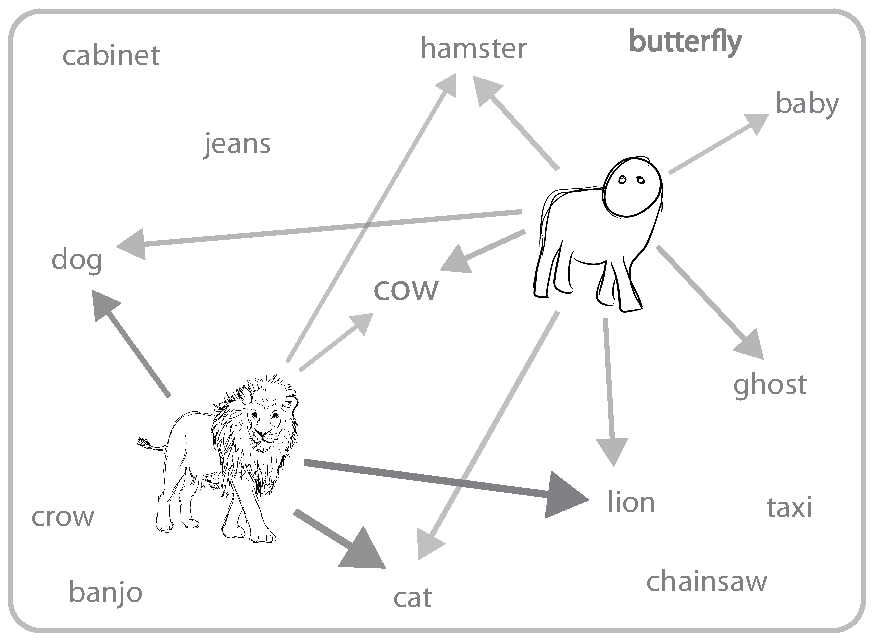
\includegraphics[width=.4\textwidth]{neurips_figures/neurips_sketch_polysemy.pdf}
%     \caption{Sketches of a ``lion'' at different levels of sparsity. More abstract depictions invite greater semantic ambiguity.}
%     \label{fig:polysemy}
% \end{wrapfigure}
However, recent evidence suggests that even high-performing vision algorithms struggle to achieve robust understanding of visual inputs that vary in their degree of abstraction \cite{baker2018abstract, singer2022photos, fan2020pragmatic}. 
One study found that current vision models trained on photorealistic image data fall short of the capabilities of the inferotemporal cortex, a key brain region supporting object categorization, in generalizing to new image distributions, including sketches.
% do not generalize as well to other image distributions, including sketches, as neurons in primate inferotemporal cortex, a key brain region supporting object categorization \cite{bagus2022primate}. 

On balance, it thus remains unclear to what degree any state-of-the-art vision algorithms achieve human-like understanding of line drawings that vary in their degree of abstraction, much less the full range of abstract images that humans regularly engage with. 
Gaining further clarity on this question requires meeting two key challenges: \textit{first}, creating a dataset containing drawings of a wide variety of object concepts that also systematically vary in their degree of abstraction; and \textit{second}, developing evaluation protocols that can be used to estimate the degree to which any model emulates \textit{human-like} understanding of this suite of drawn images.

% clear metrics to estimate the degree to which any model emulates \textit{human-like} understanding of this suite of drawn images; and \textit{third}, conducting standardized evaluations of a broad suite of current vision algorithms that permit direct comparison between them and with humans. 


\textbf{Dataset.} 
% Meeting the first challenge requires going beyond existing sketch datasets, such as \textit{TU-Berlin} \cite{eitz2012sketch}, \textit{Quickdraw} \cite{jongejan2017quick}, and \textit{Sketchy} \cite{sangkloy2016sketchy}. 
% % \cite{gryaditskaya2019opensketch,manda2021cadsketchnet}
% While all of these datasets span a reasonably wide range of visual concepts (i.e., ranging from 125 concepts in \textit{Sketchy} to 345 in \textit{Quickdraw}), none of them systematically varied how detailed individual sketches could be, one of the most straightforward ways of inducing variation in semantic abstraction \cite{berger2013style, fan2020pragmatic, yang2021visual}. 
Meeting the first challenge requires going beyond existing sketch datasets \cite{eitz2012humans, sangkloy2016sketchy, jongejan2017quick, dey2019doodle, eitz2012sketch, li2018universal, yu2016sketch, song2017deep, Gao2020SketchyCOCO, wang2019spfusionnet, sarvadevabhatla2017object, li2014comparison, li2014shrec, li2017deeper, peng2019moment, zou2018sketchyscene, liu2020scenesketcher}. 
While most of these datasets span a reasonably wide range of visual concepts (i.e., ranging from 125 concepts in \textit{Sketchy} to 345 in \textit{Quickdraw}) and some of them contain fine-grained information (e.g. stroke information and photo-sketch pairing), none of them systematically varied how detailed individual sketches could be, one of the most straightforward ways of inducing variation in semantic abstraction \cite{berger2013style, fan2020pragmatic, yang2021visual}. 
Our paper addresses the gap by providing sketches with controlled levels of detail, while encompassing the variety and granularity present in existing datasets (\autoref{tab:dataset_summary}).

\textbf{Evaluation protocol.} 
% Meeting the second challenge requires going beyond measuring model performance alone. 
Meeting the second challenge requires going beyond simple accuracy-based model performance metrics alone.
Instead, it is critical to measure detailed patterns of human behavior on the same sketch understanding tasks to evaluate how well any model emulates these behavioral \textit{patterns}, following recent work in the computational neuroscience of vision \cite{rajalingham2018large, bear2021physion, peterson2019human}.

% \textbf{Evaluations.} Meeting the third challenge requires devising an approach to conducting fair comparisons between a wide variety of models that may vary in many ways (e.g., architectural commitments, how they were trained), with the goal of guiding future model development. 

%% Introducing SEVA: Sketch-based evaluations of visual abstraction 
\vspace{-1em}
\subsection{SEVA: A Novel Sketch Benchmark for Evaluating Visual Abstraction in Humans and Machines}
\vspace{-1em}
In recognition of the above desiderata, here we introduce \texttt{SEVA} (\textbf{S}ketch-based \textbf{E}valuations of \textbf{V}isual \textbf{A}bstraction), a new sketch dataset and benchmark for evaluating alignment between human and machine visual abstraction. 

\textbf{Dataset.} Our dataset contains approximately 90K human-generated sketches of a wide variety of visual objects that also systematically vary in their level of detail, and thus the variety of meanings they evoke. 
Each sketch is associated with one of 2,048 object instances belonging to one of 128 object categories selected from the \texttt{THINGS} dataset\cite{hebart2019things}. 
We achieved variation in sketch detail by imposing constraints on how much time humans ($N$=5,563 participants) had to produce each sketch (i.e., 4s, 8s, 16s, 32s). 

\textbf{Evaluation protocol.} Leveraging these human-generated sketches, we systematically evaluated how well a diverse suite of 17 state-of-the-art vision models generate classification responses that align with those produced by humans ($N$=1,709 participants) tasked with identifying the most appropriate concept label for each sketch. 
Of these participants, 579 participants also participated in the sketch production study but were not shown any of their own sketches during this study.
We evaluated human-model alignment using three different metrics: (1) top-1 classification accuracy, reflecting raw sketch recognition performance; (2) Shannon entropy of the response distribution, reflecting the degree of uncertainty about the target label; and (3) \textit{semantic neighbor preference}, reflecting the degree to which models and humans generated off-target responses that were semantically related to the target label. 

\begin{figure}[ht!]
    \centering
    \includegraphics[width=.85\textwidth]{neurips_figures/neurips_sketchgallery_vertical_reduced.pdf}
    \caption{Humans and \texttt{CLIPasso} generated approximately 90K sketches under various production constraints.}
    \label{fig:examplegallery}
\end{figure}

\textbf{Summary of key findings.} We found that sparser human sketches produced under more severe time pressure (e.g., 4 seconds) exhibited greater \textit{semantic ambiguity}---in other words, both humans and models assigned a greater variety of labels to them than to the more detailed sketches that took more time to make (e.g., 32 seconds).
Furthermore, we found that models that better predicted human sketch recognition performance also better approximated human uncertainty about sketch meaning, but none of the models came close to approximating human response patterns to human-generated sketches at any level of detail. 
To explore the potential of models that emulate human visual abstraction in generative tasks, we conducted further evaluations of \texttt{CLIPasso}, a recently developed sketch generation algorithm \cite{vinker2022clipasso} capable of generating sketches that vary in sparsity. 
We discovered that the most detailed \texttt{CLIPasso}-generated sketches converged with human sketches of the same object concepts, as measured by the distribution of labels humans assigned to these sketches; however, sparser \texttt{CLIPasso} sketches diverged from human sketches of the same object concepts, reflecting a gap between how \texttt{CLIPasso} and human participants attempted to preserve sketch meaning under more severe production constraints. 

% represent semantic information in these sketches by benchmarking their sketch  against human behavior. 

% , for a representatively wide variety of visual object concepts varying in their degree of abstraction; 
% and (2) we systematically evaluate how well 12 diverse state-of-the-art vision models, varying in their architectures and training methods, represent semantic information in these sketches by benchmarking their recognition performance against human behavior. 
% We build on a growing body of research leveraging a global image dataset generated by the THINGS initiative \cite{hebart2019things} by sampling 2,048 real-world objects spanning 128 concepts as referents for drawings in our dataset.
% Our main goals were to test the consistency between models and humans in their ability to recognize the concepts depicted in our sketch dataset, as well as the alignment between distributions of human-generated soft labels ($N$=3,190 participants)  and distributions underlying model classification performance \cite{collins2022eliciting,peterson2019human}.
% Taken together, our work aims to contribute an informative benchmark of human and machine generated sketches spanning varying multiple levels of abstraction. 
% We hope that publicly releasing our datasets and proposed methods for investigating sketch understanding will generate opportunities for future research avenues towards building better computational models of human visual abstraction.

% \subsection{Summary of key findings}
% We found that human sketches produced under more severe time pressure (e.g., 4s) were both sparser and reliably evoked a greater variety of meanings from both humans and models than the more detailed sketches that took more time to make.
% Furthermore, we found that vision models achieving better sketch recognition performance also better approximated human uncertainty about sketch meaning, but none of the models tested provided a particularly good approximation to human response patterns to human-generated sketches at any level of detail. 
% \textbf{XXX To be continued...}

% of the world—objects, scenes, and events—at varying levels of abstraction. 
% Humans have the ability to visually communicate their knowledge of the world—objects, scenes, and events—at varying levels of abstraction. 
% could both depict scenes with incredible detail and attention towards preserving the likeness to the real world, as well as depict concepts like ``dog'' with only a single stroke by omitting much of the information that would help the sketch share a visual resemblance to a real dog. 
% The relevance and necessity to abstract visually across many different levels arises across many instances of visual communication.
% In certain contexts, a faithful and detailed depiction might be what is required, such as when an architect conveys detailed schematics to an engineer \cite{suwa1997architects} or when a zoologist creates scientific illustrations of a new animal species \cite{baigrie1996picturing}. 
% However in other contexts, such as when there exists established social conventions or when resources are limited (e.g., time), simpler depictions can be used to efficiently denote objects \cite{fan2020pragmatic, garrod2007foundations, hawkins2021visual}. 
% Amongst these cases, one tool for visualization that might showcase the greatest variability in visual abstraction while being widely pervasive are line drawings \cite{sayim2011line}.

\vspace{-0.5em}
\section{Methods}
\vspace{-0.5em}
\subsection{Human Sketch Production}
\vspace{-0.5em}
A core contribution of this work is a new dataset containing human-generated sketches of a wide range of visual object concepts that also systematically span multiple levels of semantic abstraction. 
We created this dataset by crowdsourcing these sketches online, following prior work \cite{fan2018common, yu2016sketch, sangkloy2016sketchy, fan2020pragmatic, hawkins2023visual, jongejan2017quick}.
Each sketch in the dataset was recorded as a bitmap image as well as a collection of stroke coordinates, thus preserving the precise cursor movements a participant enacted to create the sketch.

\textbf{Participants.} 
5,563 participants (2,870 male; $M_{age}$ = 36.7 years) were recruited from Prolific and compensated $\$15.50$/hour for their participation.
Data from 104 of these sessions were excluded from subsequent analyses due to technical issues (e.g., images did not load). 
% We excluded data from 104 sessions due to technical glitches.
All participants provided informed consent in accordance with the UC San Diego IRB.
% our university's IRB (blinded for review). % 

\textbf{Object concepts.} We included 128 concrete real-world object categories (e.g., ``lion'', ``banjo'', ``car'') sourced from the \texttt{THINGS} dataset. 
We used the \texttt{THINGS} dataset \cite{hebart2019things, hebart2023things} because it is a well validated set of concrete, real-world visual object categories designed to support interoperability among large-scale studies in human visual cognition and cognitive neuroscience.
% Building on a prior study investigating human sketch production at different levels of abstraction \cite{yang2021visual}, we sampled concepts from the entire library of 1,854 concepts based spanning four main axes of variation: familiarity, artificiality, animacy, and size. 
For each of these 128 object concepts, we randomly sampled 16 object instances represented by color photographs, which served to visually ground the human sketch production task. 
As such, each sketch in our dataset is uniquely associated with one of these 2,048 object instances, and our final sample size was determined by our predefined goal of obtaining at least 10 human sketches of each of these instances. 
% color photographs furnishing a final set of 2,048 instance photographs, which served as referents for the human sketch production task.
% 2,048 images
% \subsection{Human sketch production Task}

\begin{table}[htp!]
\resizebox{\textwidth}{!}{%
% \begin{tabular}{@{}llllll@{}}
% \toprule
% \textbf{Dataset Name} & \textbf{Dataset Contents} & \textbf{\# Classes} & \textbf{Stroke Info?} & \textbf{Photo Cue?} & \textbf{Abstraction?} \\ \midrule
% TU-Berlin~\cite{eitz2012humans}   & 20K sketches & 250 & \checkmark  & & \\
% QuickDraw~\cite{jongejan2017quick} & 50M+ sketches & 345  & \checkmark  & & \\
% SPG ~\cite{li2018universal} & 20K sketches & 25 & \checkmark & &\\
% SketchSeg-10K~\cite{wang2019spfusionnet}  & 10K sketches  & 10 & & & \\
% SketchFix-160~\cite{sarvadevabhatla2017object} &  3.904K sketches  & 160  & \checkmark  & &  \\
% Sketchy~\cite{sangkloy2016sketchy}     & 75K sketches, 12K photos  & 125  &  \checkmark &  \checkmark & \\
% QMUL~\cite{yu2016sketch, song2017deep} & 1.284K sketches, 1284 photos  & 3  &    & \checkmark & \\
% QuickDrawExtended~\cite{dey2019doodle}  & 330K sketches, 204K photos & 110   &  & & \\
% SBSR~\cite{eitz2012sketch} & 1.814K sketches, 1814 3D models & 161  &  & &\\
% SHREC'13~\cite{li2014comparison} & 7.2K sketches, 1258 3D models & 90  &  &   & \\
% SHREC'14~\cite{li2014shrec}   & 12.68K sketches, 8987 3D models & 171  &    & &\\
% PACS DG~\cite{li2017deeper} &  9.991K sketches, photos, cartoons, paintings  &  7 & & & \\
% DomainNet~\cite{peng2019moment}  & 600K sketches, photos, paintings, and others & 345  & & & \\
% SketchyScene~\cite{zou2018sketchyscene} & 29K sketches, 7K photos  & N/A  & & & \\
% SketchyCOCO~\cite{Gao2020SketchyCOCO} &  14K+ sketches, photos, edge-maps  & 17  & \checkmark  &\checkmark & \\
% SceneSketcher~\cite{liu2020scenesketcher} &  1.225K scene sketch-photo pairs  & 14  & \checkmark  & \checkmark& \\
% \textbf{SEVA} & \textbf{90K sketches, 2048 photos} & \textbf{128} & \checkmark  & \checkmark & \checkmark  \\ \bottomrule
% \end{tabular}%
\begin{tabular}{@{}llllll@{}}
\toprule
\textbf{Dataset Name} & \textbf{Dataset Contents} & \textbf{\# Classes} & \textbf{Stroke Info?} & \textbf{Photo Cue?} & \textbf{Abstraction?} \\ \midrule
TU-Berlin~\cite{eitz2012humans}   & 20K sketches & 250 & \checkmark  & & \\
QuickDraw~\cite{jongejan2017quick} & 50M sketches & 345  & \checkmark  & & \\
QuickDrawExtended~\cite{dey2019doodle}  & 330K sketches, 204K photos & 110   &  & & \\
SPG ~\cite{li2018universal} & 20K sketches w/ stroke grouping & 25 & \checkmark & &\\
SBSR~\cite{eitz2012sketch} & 1.8K sketches, 1.8K 3D models & 161  &  &  &\\
QMUL~\cite{yu2016sketch, song2017deep} & 1.3K sketches, 1.3K photos  & 3  &    & \checkmark & \\
Sketchy~\cite{sangkloy2016sketchy}     & 75K sketches, 12K photos  & 125  &  \checkmark &  \checkmark & \\
SketchyCOCO~\cite{Gao2020SketchyCOCO} &  14K sketches, 14K photos  & 17  & \checkmark  &\checkmark & \\
\textbf{SEVA} & \textbf{90K sketches, 2048 photos} & \textbf{128} & \checkmark  & \checkmark & \checkmark  \\ \bottomrule
\end{tabular}%
}
\caption{Comparison between SEVA and prior sketch datasets.}
\label{tab:dataset_summary}
\end{table}
% DomainNet: ClipArt, infographics, paintings, QuickDraw, real photos, professional sketches


\textbf{Sketch production task.} In each session, participants produced sketches of 16 different object categories, randomly sampled from the full set of 128 object categories.
On each trial, they were cued with a color photograph (500px x 500px) of an object paired with its concept label. 
Each participant was randomly assigned to one of four conditions, defined by the maximum amount of time participants could take to produce their sketches: 4 seconds, 8 seconds, 16 seconds, or 32 seconds (Fig.~\ref{fig:examplegallery}, \textit{left}). 
Such random assignment of participants to condition ensures that estimates of differences between conditions will not, in expectation, be biased by individual differences in sketching behavior.
% \edited{We chose a between-subjects randomization, because we predicted that it would be easier for participants to produce sketches within the same time constraint across all 16 sketches rather than adjusting to new a time constraint for each sketch.}
Participants drew on a digital drawing canvas (500px x 500px) using whatever input device they already had available (e.g., mouse, stylus) and were able to undo their most recent stroke or completely clear their canvas if needed. 
They were encouraged to make their drawings as recognizable as they could at the concept level and to use the photograph only to remind them of what individual objects belonging to that category generally look like.  
A countdown timer indicated how many seconds they had left to produce their drawing. 
Each trial ended either when time ran out or when the participant indicated that they wished to continue to the next trial, but participants were encouraged to use the full time available to produce as recognizable of a drawing as they could.
At the beginning of the session, participants were explicitly instructed not to include any background context (e.g., grass in a drawing of a ``horse''), arrows, or text.
Participants also completed one practice trial (that we did not include in analyses) at the beginning of the session to familiarize themselves with the drawing interface.
Our final dataset contains 89,797 sketches after filtering out invalid sketches (e.g., blank canvases).



\subsection{Human Sketch Understanding}
\vspace{-1em}
A key component of any evaluation of how well current vision algorithms emulate human visual abstraction is measurement of human behavior in tasks relying on visual abstraction. 
Here we focus on characterizing what meanings humans extract from the collected sketches, providing the basis for our subsequent empirical evaluation of how well any state-of-the-art vision model approximates human response patterns when presented with the same sketches.  

% In order to benchmark vision algorithms on their ability to understand the semantic content represented in sketches, we aimed to establish recognizability baselines for each sketch by acquiring dense soft-label human judgements \cite{collins2022eliciting,collins2023human, peterson2019human} for a subset of sketches produced in the previous experiment. 

\vspace{1em}
\textbf{Participants.}
1,709 participants (776 male; $M_{age}$ = 39.2 years) were recruited from Prolific and compensated $\$15.50$/hour for their participation. % were recruited to make recognition judgments on the 8,192 sketches.
Data from 21 of these sessions were excluded from subsequent analyses due to technical issues.
% We excluded 28 data sessions from participants who experienced technical difficulties. 
Our predefined criterion for stopping data collection was acquisition of at least 12 recognition judgments for each sketch. 


\textbf{Sketch recognition task.}
In each session, participants provided labels for 64 sketches randomly sampled from a fixed set of 8,192 sketches, approximately 10\% of the full human sketch dataset. 
The specific set of 8,192 sketches included in this experiment was determined by randomly sampling one sketch cued by each object instance from each drawing-time condition (i.e., 16 instances/concept x 128 categories x 4 drawing-time conditions = 8,192). 
On each trial, participants were presented with a single sketch (300px x 300px) and a text field where they could provide their best guess concerning the concept the sketch was intended to convey. 
As soon as they began typing, a dropdown menu appeared with suggested word completions.
This dropdown menu contained the entire set of 1,854 labels in the \texttt{THINGS} dataset and only responses that matched one of these 1,854 labels were accepted. 
Because many words have multiple meanings, the labels contained in this dropdown menu were also accompanied by disambiguating text (e.g., to distinguish \textit{mouse (animal)} from \textit{mouse (computer)}). 
If participants were unsure of which label best applied to the sketch, they were encouraged to provide additional guesses (up to 5 per sketch). % , though in practice participants provided these additional guesses on only \textbf{YY\%} of trials
Collecting multiple labels on each drawing trial was important because it enabled us to more thoroughly sample the distribution of meanings that each sketch evoked for human participants (i.e., which labels came to mind and how often they did so). 
At the beginning of the session, participants completed a practice trial (that we did not include in analyses) to familiarize themselves with the labeling interface.
% To assess whether participants were fully engaged with the task, they also completed an attention-check trial in the middle of the experiment. 

% (Fig. \ref{fig:VAB_polysemy}, \textit{left})
% To accomplish this, we designed a web-based recognition study, where participants could provide multiple object labels per sketch from the entire library of 1,854 THINGS object labels.
% Curating multiple soft labels was critical insofar that sketches often capture a range of semantic meaning and can bring to mind many possible concepts during viewing (Fig. \ref{fig:VAB_polysemy}, \textit{left}). 
% Human provided soft labels allowed us to represent the semantic content of a sketch as a probability distribution over all possible labels.
% We collected recognition judgements for a sample of 8,192 of the sketches from the human sketch production study.  
% This sample contained 16 different sketches of each of the 128 classes produced under the 4 different time constraint conditions (16 $\times$ 128 $\times$ 4).

% Each participant was presented with a randomized series of 64 sketches from the set of  8,192 subsampled sketches (300px x 300px). 
% On every trial, they were presented with a single drawing and a text box and asked to provide a label that best represented the drawing by typing their response into the box. 
% Upon beginning to type, participants were presented with a drop-down menu that displayed a subset of the 1,854 THINGS object concepts that had string matches to the participant's typed response.
% Each label also had words within parentheses to eliminate ambiguity (e.g. \textit{mouse (animal)} was a different label than \textit{mouse (computer)}). 
% The participant could choose from one of these options to label the sketch.
% Participants could also add up to 5 additional text boxes to submit multiple labels if they believed a sketch was representative of multiple object concepts, but were not permitted to submit custom label options not included in the 1,854 labels. 
% A trial ended when participants were satisfied with their selected label(s) and pressed a “Submit” button.
% Prior to test trials, participants completed a practice trial to familiarize themselves with the labeling interface. 



\subsection{Machine Sketch Understanding}

We propose a generic protocol for evaluating machine sketch understanding that can be applied to any vision algorithm using our sketch dataset. 
In this paper, we conduct evaluations of a wide range of state-of-the-art vision models with the goal of demonstrating the feasibility of our protocol and guiding future model development. 

\textbf{Model suite.} Specifically, we evaluated 17 vision models spanning a wide range of architectures and training methods (Table \ref{tab:models}), all of which have been demonstrated to achieve high performance on object recognition on standard datasets, such as ImageNet \cite{deng2009imagenet}. We also made sure to include variants of standard ConvNet and Transformer models that have gained traction within the field of computational cognitive neuroscience for their potential to close the gap between biological and artificial vision \cite{konkle2021beyond,fel2022aligning,kubilius2019brain,mehrer2021ecologically}.



\begin{table}[htp!]
\centering

\resizebox{.9\textwidth}{!}{%
\begin{tabular}{@{}llll@{}}
\toprule
\textbf{Model}  & \textbf{Architecture} & \textbf{Training Paradigm} & \textbf{Dataset}\\ 
\midrule
\textbf{\textcolor{VGG-19}{VGG-19}}~\cite{simonyan2014very} & VGG-19 & supervised & ImageNet \\ 
\textbf{\textcolor{Inception-V3}{Inception-V3}}~\cite{szegedy2016rethinking} & Inception-V3 & supervised & ImageNet\\
\textbf{\textcolor{ResNet-50}{ResNet-50}}~\cite{he2016deep} &  ResNet-50  & supervised & ImageNet\\
\textbf{\textcolor{ViT-B}{ViT-B}}~\cite{dosovitskiy2020image} & ViT-B & supervised & ImageNet\\
\textbf{\textcolor{Swin-B}{Swin-B}}~\cite{liu2021swin} & Swin-B & supervised & ImageNet\\
\textbf{\textcolor{MLPMixer-B}{MLPMixer-B}}~\cite{tolstikhin2021mlp} & MLPMixer-B & supervised & ImageNet\\
\textbf{\textcolor{CORnet-S}{CORnet-S}}~\cite{kubilius2019brain} & CORnet-S & supervised & ImageNet\\
\textbf{\textcolor{Harmonization}{Harmonization}}~\cite{fel2022aligning} & ViT-B & supervised & ImageNet + Human Feature Importance~\cite{fel2022aligning}\\
\textbf{\textcolor{ECOSET}{ECOSET}}~\cite{mehrer2021ecologically} & ResNet-50 & supervised & ECOSET~\cite{mehrer2021ecologically}\\
% \textbf{\textcolor{MoCo-v2}{MoCo-v2}}~\cite{chen2020improved} & ResNet-50 & self-supervised \\
\textbf{\textcolor{SimCLR}{SimCLR}}~\cite{chen2020simple} & ResNet-50 & self-supervised & ImageNet\\
\textbf{\textcolor{MoCo-v3}{MoCo-v3}}~\cite{chen2021empirical} & ViT-B & self-supervised & ImageNet\\
\textbf{\textcolor{DINO}{DINO}}~\cite{caron2021emerging} & ViT-B & self-supervised & ImageNet\\
% \textbf{\textcolor{DINO}{DINO}}~\cite{caron2021emerging} & ResNet-50 & self-supervised & ImageNet\\
\textbf{\textcolor{MAE}{MAE}}~\cite{he2022masked} & ViT-B & self-supervised & ImageNet\\
\textbf{\textcolor{CLIP}{CLIP}}~\cite{radford2021learning} & ViT-B & self-supervised & WebImageText~\cite{radford2021learning}\\
\textbf{\textcolor{IPCL}{IPCL}}~\cite{konkle2021beyond} & AlexNet & self-supervised & ImageNet\\
\textbf{\textcolor{Noisy Student}{Noisy Student}}~\cite{xie2020self} & EfficientNet-b4 & semi-supervised & ImageNet + JFT~\cite{sun2017revisiting}\\
\textbf{\textcolor{SWSL}{SWSL}}~\cite{yalniz2019billion} &  ResNet-50  & semi-supervised & ImageNet + YFCC-100M~\cite{thomee2016yfcc100m} + IG-1B-Targeted~\cite{yalniz2019billion}\\
\bottomrule 
\end{tabular}%
\\
}
\vspace{1em}
\caption{Model suite annotated by backbone architecture, training paradigm, and training dataset.}
\vspace{-1em}
\label{tab:models}
\end{table}


% We performed all our computations on latent features extracted from the deepest (non-fully-connected) layers of these models, which amounted to extracting activation patterns at either the model's final convolution or attention layer.




\textbf{Evaluation Protocol.}
The goal of our evaluation protocol was to measure how well any of these vision models approximated human sketch recognition behavior when presented with the same sketches. 
Because these models contain different latent representations of widely varying dimensionalities, we measured machine sketch-recognition behavior by extracting activation patterns from each model's final convolutional or attention block and training linear classification-based readouts on these activation patterns. 
That is, for each model we independently fit 1,854-way logistic regression classifiers using 5-fold stratified cross-validation to predict the ``ground-truth'' concept label associated with each sketch.
\footnote{Because these classification-based readouts were only trained on sketches of 128 object concepts subsetted from the \texttt{THINGS} dataset, the probabilities assigned to the remaining 1,726 labels were set to zero during training. As such, none of these models produced any of these other labels at test time, but humans in the sketch recognition experiment \textit{could} select these other labels. This difference between how sketch recognition behavior was elicited from humans and models led us to focus on relative measures of performance when evaluating human-model alignment.} 

% That is, for each model we independently fit 128-way logistic regression classifiers using 5-fold stratified cross-validation to predict the ``ground-truth'' category label from the feature embeddings of each sketch.
% \footnote{Because these classification-based readouts were only trained on sketches of 128 object concepts subsetted from the \texttt{THINGS} dataset, they never predicted any of the remaining 1,726 category labels. But humans in the sketch recognition experiment \textit{could} may select any label from the 1,854 labels. This difference between how sketch recognition behavior was elicited from humans and models led us to focus on relative measures of performance when evaluating human-model alignment.} 

These predicted labels were aggregated across the 16 sketches of the same concept (e.g., \textit{lion}) and from the same drawing-time condition (e.g., 4 seconds) to yield a model's response distribution for that \textit{type} of sketch.
The top-1 classification accuracy was determined by computing the relative frequency of the ``ground-truth'' concept label in this response distribution. 
We also computed the Shannon entropy of this response distribution to estimate the degree of semantic ambiguity exhibited by this type of sketch.
Further, we derived a measure of the degree to which even the \textit{non-}ground-truth labels generated by each model were semantically related to the ground-truth label, which we term the \textit{semantic neighbor preference} score.
This semantic neighbor preference score falls in the range $[0,1]$ and is highest when labels that are more semantically related to the ground-truth label appear more frequently than more semantically distant labels, is close to 0.5 when labels appear with uniform probability, and is minimized when labels that are more semantically distant appear most frequently. 

To compare model classification outputs with human responses, we derived an analogous response distribution from the human labels obtained in the human sketch recognition experiment. 
That is, we aggregated all labels assigned by human participants to all 16 sketches of the same concept (e.g., \textit{lion}) and from the same drawing-time condition (e.g., 4 seconds) to construct a response distribution for each type of sketch. 
We then computed the same three metrics above (i.e., top-1 classification accuracy, response entropy, semantic neighbor preference) using the human response distributions. 

% we leveraged the label data generated from our recognition study to compute the number of times each of the 1,854 labels was assigned to a given sketch.
% By summing these label counts across participants and normalizing them, we generated a human recognition ``response'' vector for each sketch, representing a distribution over the 1,854 labels as a measure of its perceived polysemy. 
% Importantly, this provided an analogous baseline of comparison to the class probability vectors extracted from the classifiers.

% People can recognize both a detailed and sparse sketch of Picasso's bulls as a bull. 
% Are vision models also able to decode the semantic information conveyed in a drawing despite its level of abstraction?
% Here, we outline a protocol for testing this hypothesis.
% Here, we outline a standard procedure for evaluating any image-computable visual encoder on its sensitivity to varied visual abstraction. 
% Our approach is to measure the recognition performance and class label uncertainty expressed by any vision model and evaluate these metrics against comparable measures from our human sketch recognition task.
% Due to the varied dimensionality and characteristics of the latent model features (outputs of convolution vs. attention layers vs. linear layers), in order to fairly assess the semantic information decodable from these features, we fit a series of regularized logistic classifiers predicting the class labels of each sketch from model latent features.
% Classifiers were fit separately to each vision model's latent features using 5--fold stratified cross-validation to predict the class label of the sketch. 
% For each sketch, when presented in the test fold, we preserved the full vector of class probabilities corresponding to the 1,854 THINGS object classes. It is worth noting that while the true identity of the sketches belonged to only 128 classes, since humans were allowed to provide labels from the entire set of 1,854 concept labels we set the probability values of the non-represented concepts to 0.
% Next, to compare these model data against human recognition, we leveraged the label data generated from our recognition study to compute the number of times each of the 1,854 labels was assigned to a given sketch.
% By summing these label counts across participants and normalizing them, we generated a human recognition ``response'' vector for each sketch, representing a distribution over the 1,854 labels as a measure of its perceived polysemy. 
% Importantly, this provided an analogous baseline of comparison to the class probability vectors extracted from the classifiers.
% The spread of these label distributions  for a given sketch can be taken as a measure of its perceived polysemy over the 1854 labels

\subsection{Machine Sketch Production}

To explore the potential of models that emulate human visual abstraction in generative tasks, we also include evaluations of \texttt{CLIPasso}, a recently developed sketch generation algorithm \cite{vinker2022clipasso} capable of generating sketches that vary in sparsity.

\textbf{Generating machine sketches.} Specifically, we leveraged \texttt{CLIPasso} to generate 8,192 sketches conditioned on the same 2,048 object instances we used in the human sketch production experiment such that each sketch was constrained to consist of either 4, 8, 16, or 32 pen strokes (Fig.~\ref{fig:examplegallery}, \textit{right}). 
\texttt{CLIPasso} generates sketches by optimizing the parameters of a set of curves (i.e., start/end points; control points), each representing a single pen stroke, to be similar to target image.
This optimization is guided by a pretrained implementation of CLIP \cite{radford2021learning}, a large model trained using contrastive learning on vast quantities of text-image pairs.
Similarity to the target image is defined based on the distance between CLIP's embedding of the target image and its embedding of the sketch, where these embeddings reflect combinations of feature activations from multiple intermediate layers of CLIP. 

\textbf{Measuring human understanding of machine sketches.} We evaluated human recognition performance on these \texttt{CLIPasso}-generated sketches by recruiting 1,481 participants (730 male; $M_{age}$ = 41.05 years) on Prolific to complete the same sketch recognition task described earlier.
Data from 7 of these sessions were excluded from subsequent analyses due to technical issues.

% We excluded 28 participants who experienced technical difficulties.

% in intermediate layer activations on both the input image and the sketch.
% The abstraction degree is controlled by varying the number of strokes. 
% To investigate this observation, we utilize CLIPasso \cite{vinker2022clipasso}, a recently introduced method that generates sketches of objects at various abstraction levels.
% In CLIPasso, a sketch is represented as a set of parametric curves (strokes), whose parameters are optimized to depict a given image.
% The optimization is guided by a pretrained CLIP model, leveraging its powerful semantic and visual priors. 
% A CLIP-based loss is defined between the input image and the rasterized sketch, based on the distance between CLIP's latent embedding and its intermediate layer activations on both the input image and the sketch.
% The abstraction degree is controlled by varying the number of strokes. 

% We used CLIPasso to generate 8,192 sketches — one sketch for each of the 16 photographs in each of the 128 concept categories at 4 levels of abstraction (16 $\times$ 128 $\times$ 4).
% Because CLIPasso varies detail by modulating the number of strokes in a given sketch, to mirror the human sketch production task as closely as possible, we generated sketches using 4, 8, 16, and 32 strokes.

% \subsection{Statistical Analyses} Throughout this paper, we estimate the impact of our manipulation of drawing time and differences between models by fitting mixed-effects regression models, with random intercepts for different object concepts. 

\begin{wrapfigure}{r}{0.5\textwidth}
    \centering
    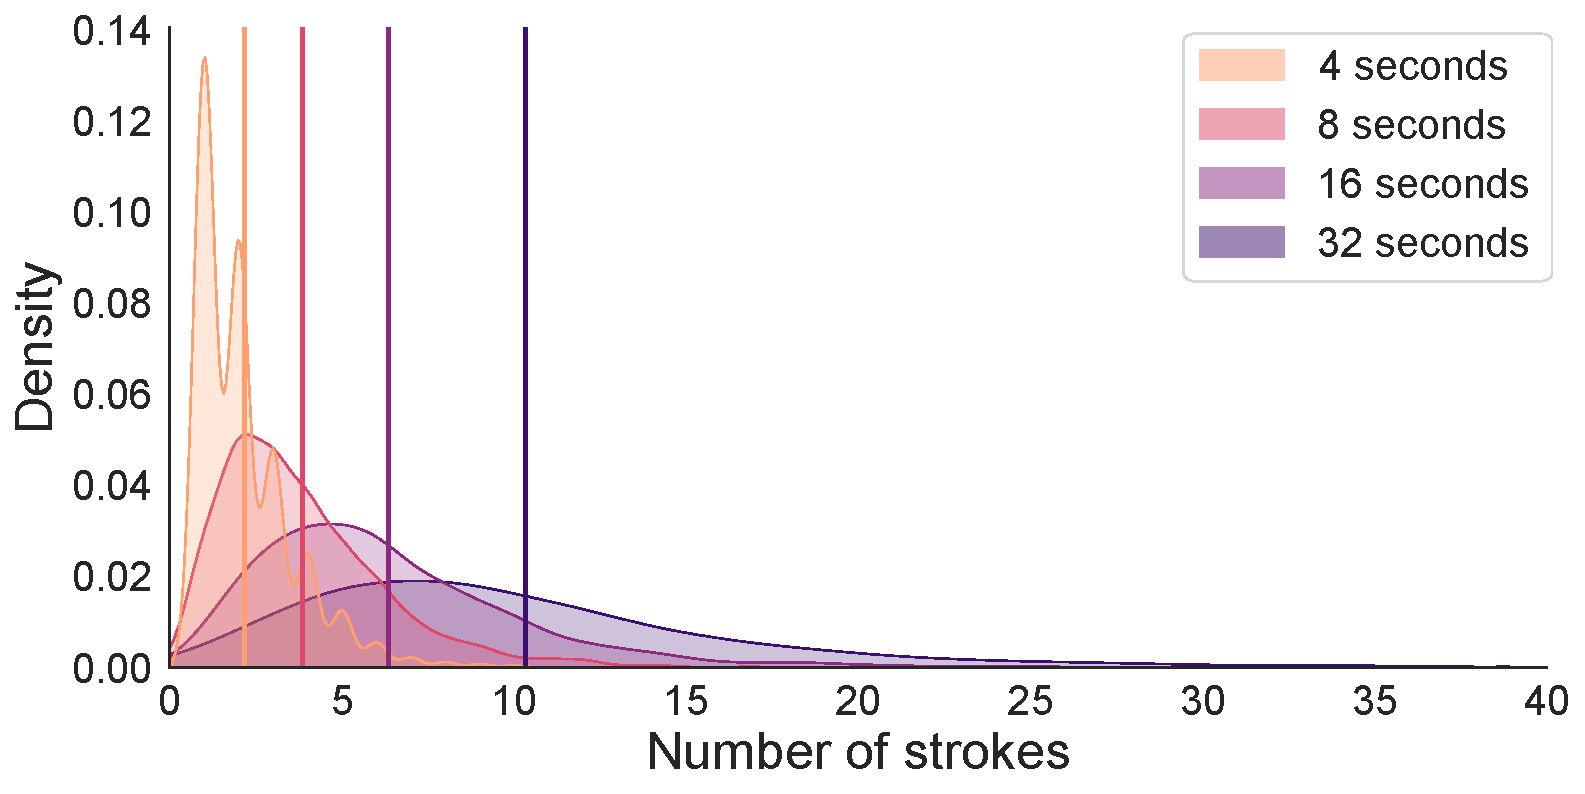
\includegraphics[width=.5\textwidth]{neurips_figures/neuripsDB_stroke_complexity_by_dd_edited.pdf}
    \caption{Distributions of number of strokes for each drawing time condition in the human sketch production task. Vertical lines indicate means.}
    \label{fig:dd_v_numstrokes}
    \vspace{-1em}
\end{wrapfigure}

\section{Results}
% \subsection{Benchmarking machine sketch understanding}


% Throughout, we estimate the impact of our manipulation of drawing time and differences between models by fitting mixed-effects regression models, with random intercepts for different object concepts. 

\textbf{Humans produce sparser sketches under stronger time constraints.}
We first sought to validate the effect of manipulating the maximum time that human participants had to draw on how detailed their sketches were. 
We estimated how detailed a sketch was by counting the number of strokes it contained (Fig.~\ref{fig:dd_v_numstrokes}) and then fit a mixed-effects linear regression model predicting the number of strokes as a function of drawing-time condition (i.e., 4s, 8s, 16s, 32s), with random intercepts for object concept.
We found that drawings produced under the 4s limit contained the fewest strokes on average, whereas those produced under the 32s limit contained the greatest number of strokes ($\beta=.29$, $SE=4.95 \times10^{-3}$, $p<.001$).
These results confirm that restricting the amount of time human participants had to produce their sketches led to systematic differences in how detailed their sketches were.
% These differences are critical for measuring human and model sensitivity and robustness to variable visual depictions of the same underlying object concept.

% % \vspace{-1em}
% \begin{figure*}
%     \centering
% 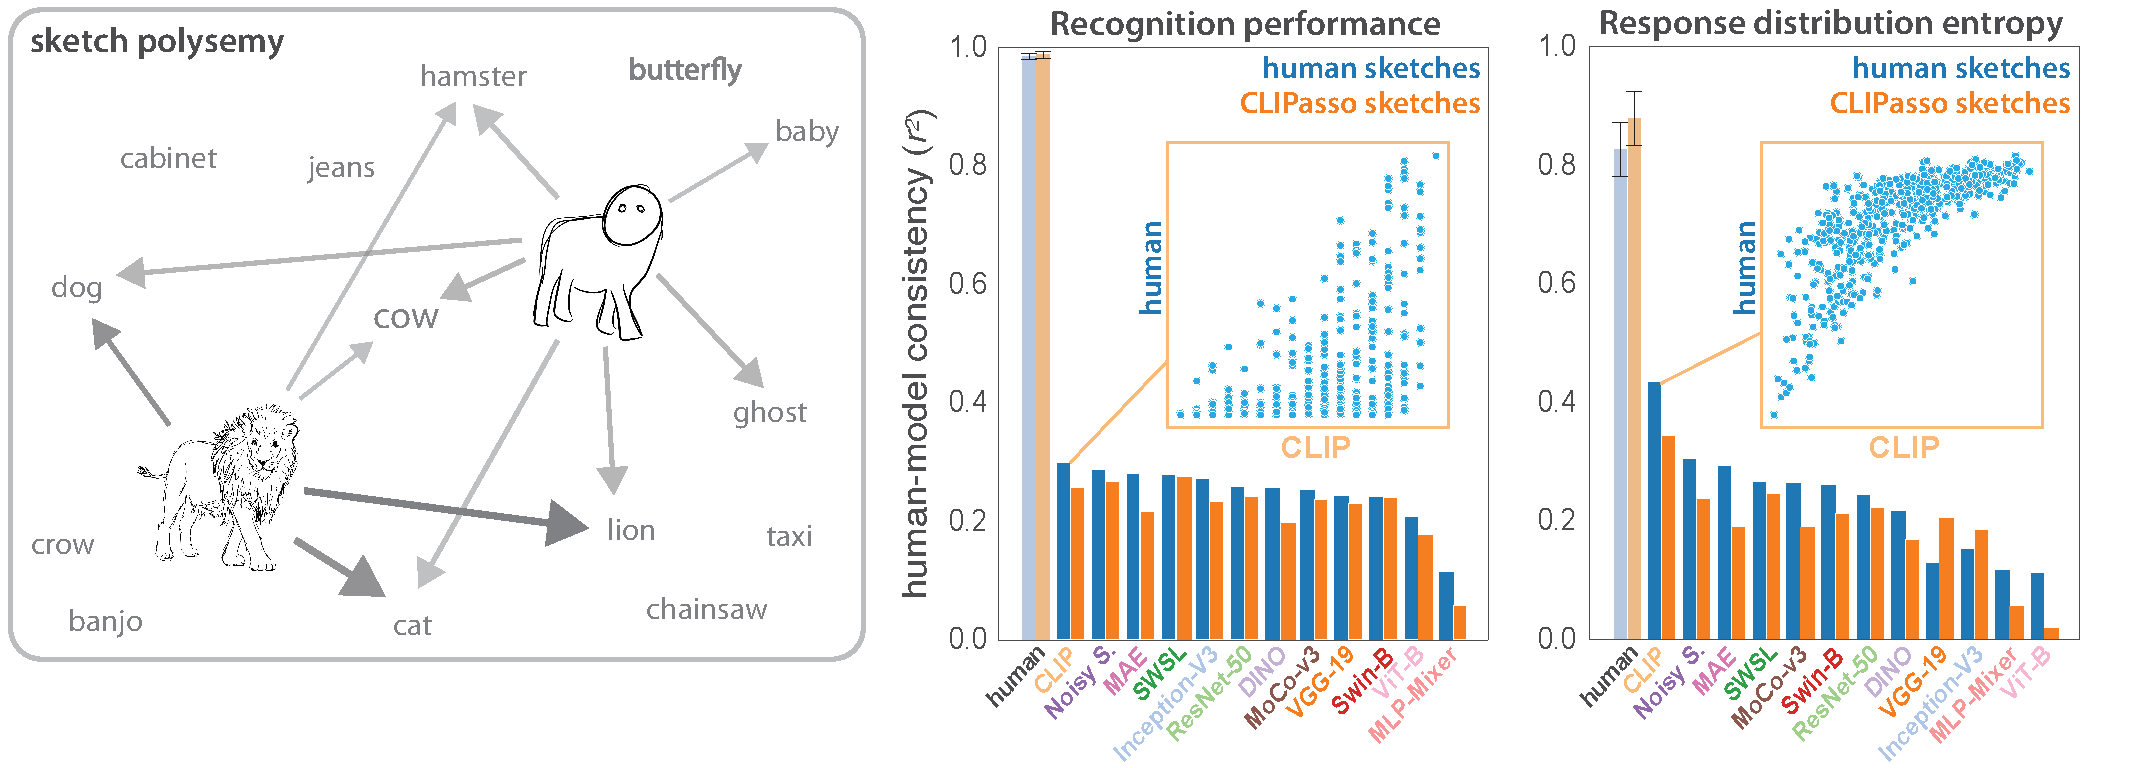
\includegraphics[width=1\linewidth]{figures/VAB_polysemy_no_mocov2.pdf}
%     % \vspace{-1em}
%     \caption{\textit{Left:} Example of sketch polysemy at different levels of abstraction. \textit{Middle:} Proportion of variance explained in top-1 human recognition accuracy by model top-1 accuracy. \textit{Right:} Proportion of variance explained in human response distribution entropy by model class probability entropy. Inset scatterplots show the distribution of entropy values between human judgements and CLIP.}
%     \vspace{-1em}
%     \label{fig:VAB_polysemy}
% \end{figure*}
% % \subsubsection{Varying stroke complexity and draw duration  moderates perceived semantics in sketches for both humans and machines.}

\begin{table}[t!!]
    \centering
    \resizebox{.9\textwidth}{!}{
    \begin{tabular}{l|l|l||l|l||l|l}
    time & accuracy$_{mean}$ & accuracy$_{sem}$& entropy$_{mean}$ & entropy$_{sem}$& SNP$_{mean}$ & SNP$_{sem}$\\
    \toprule
        \textbf{4 seconds} & .031 & .003 & 1.958 & .011 & .628  & .008\\
        \textbf{8 seconds} & .082 & .004 & 1.814 & .013 & .701 & .009\\
        \textbf{16 seconds} & .139 & .006 & 1.690 & .014 & .750 & .010\\
        \textbf{32 seconds} & .199 & .007 & 1.555 & .015 & .787 & .010\\
        \bottomrule
      
    \end{tabular}}\\\
    \caption{Human sketch understanding under each draw duration constraint. Columns represent means and standard errors of the mean for top-1 accuracy, response entropy, and semantic neighbour preference (SNP).}
    \vspace{-2em}
    \label{tab:human_performance}
\end{table}



\textbf{Sparser sketches are more semantically ambiguous for models and humans.}
Having verified that we had successfully manipulated the level of detail in human sketches, we next sought to evaluate how well current vision models extract semantic information from them at each level of detail. 
Our general approach was to fit mixed-effect linear regression models to estimate the effect of sparsity on 3 key metrics: (1) top-1 classification accuracy, (2) entropy of response distributions, and (3) semantic neighbor preference. Regression models included random intercepts and slopes for object concepts.
Figure \ref{fig:accuracy_entropy_snp} shows the performance of each vision model with respect to these metrics for sketches produced under different time constraints.

% We also estimated whether different vision models had comparable performance with respect to each of these metrics. 
We found that models generally achieved higher top-1 classification accuracy for more detailed sketches than sparser ones ($\beta=9.57\times10^{-2}$, $t=20.25$, $p<.001$).
\begin{wrapfigure}{r}{.35\textwidth}    
    \centering
    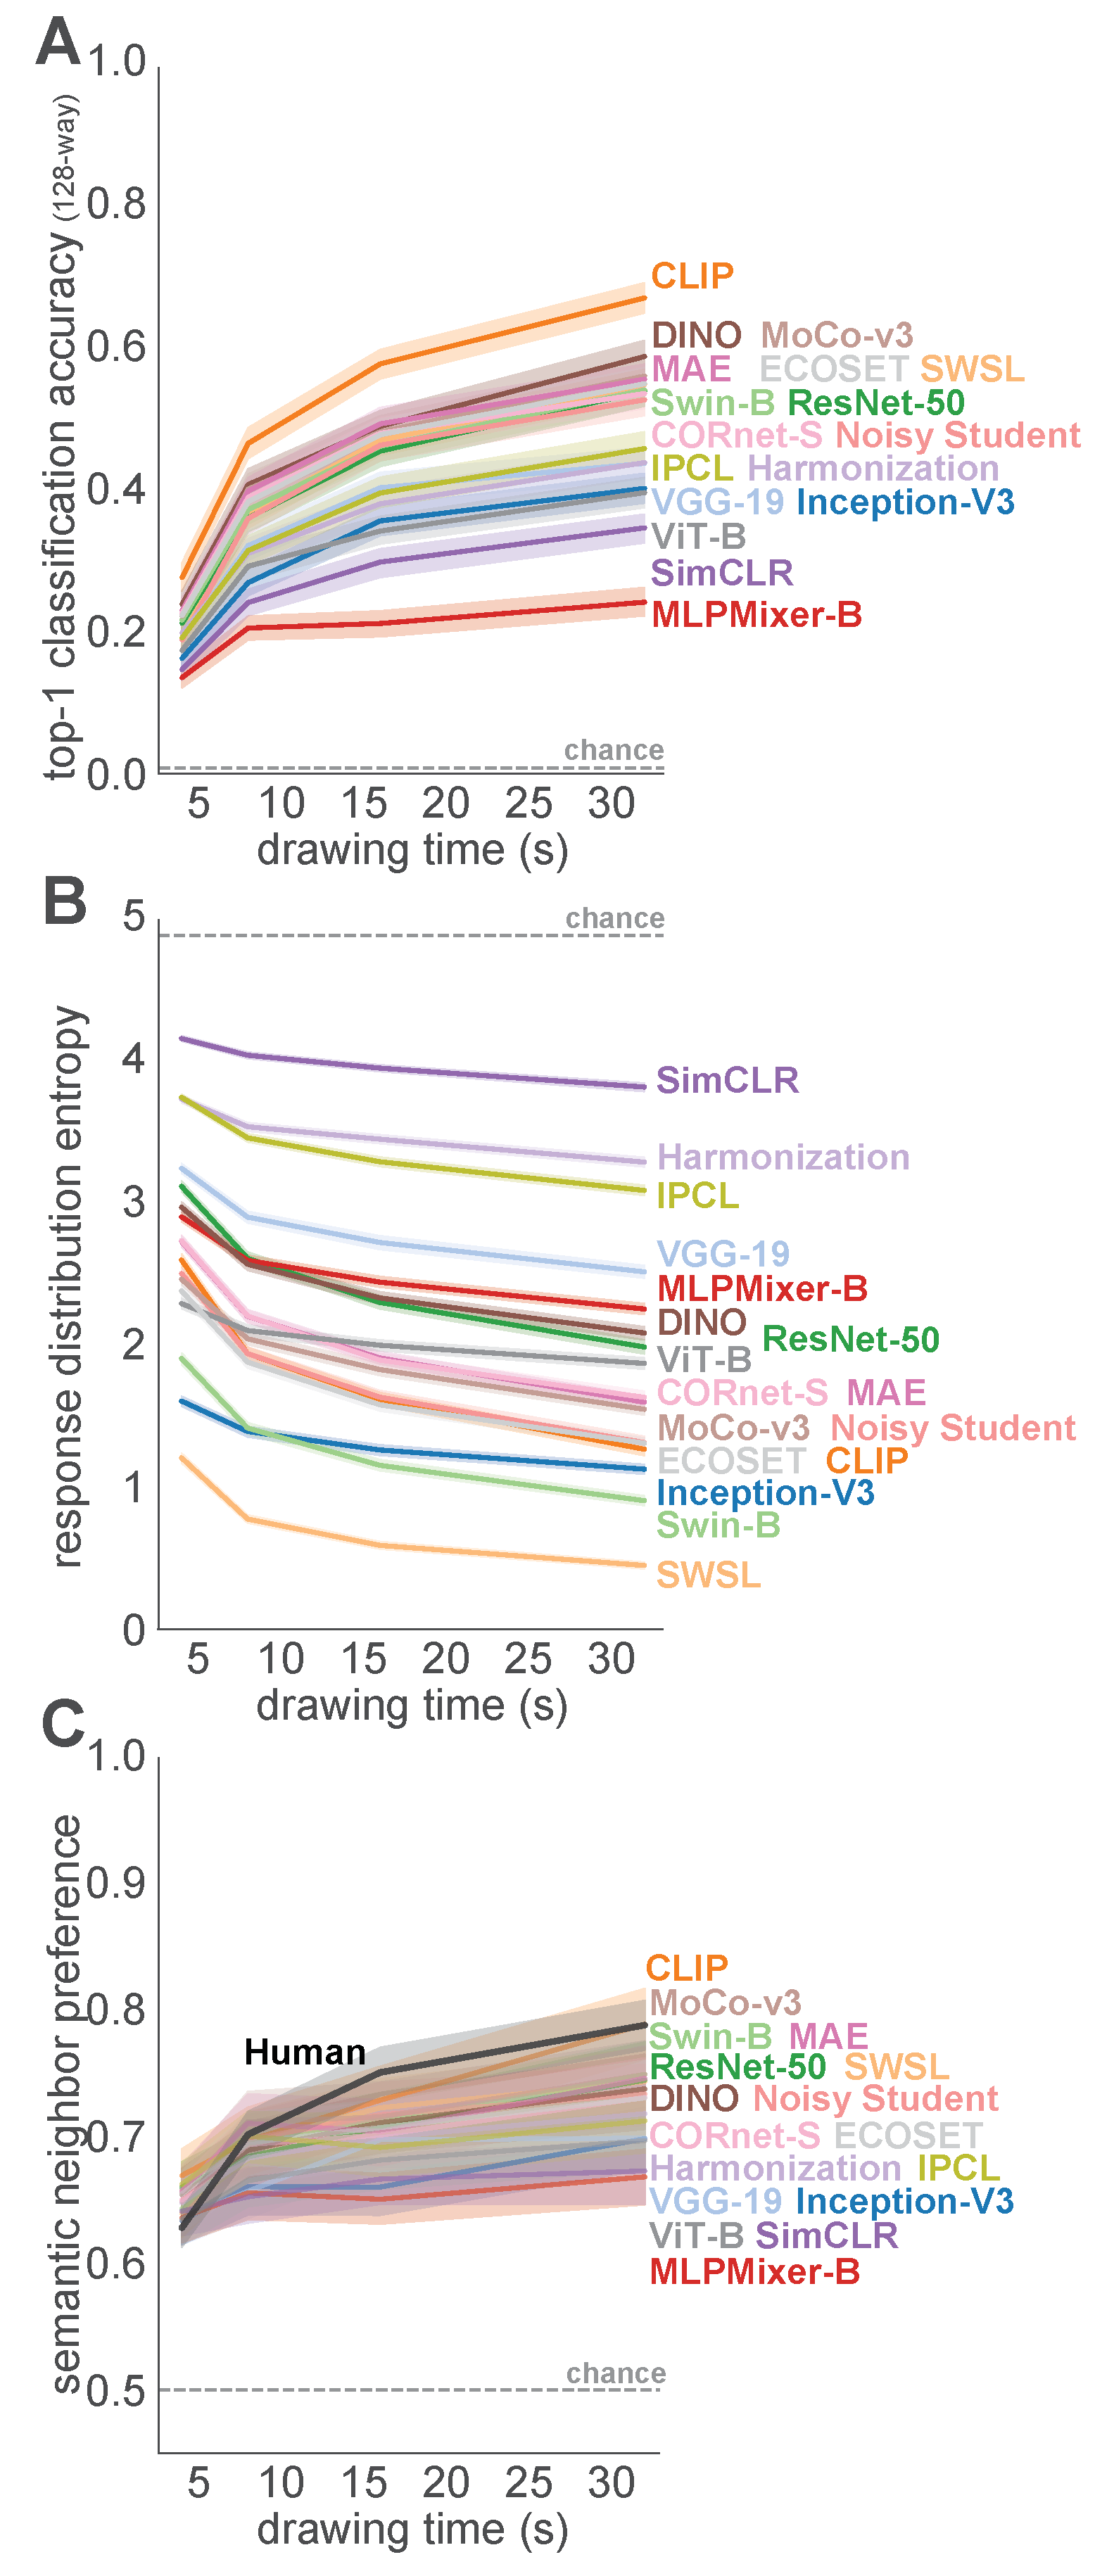
\includegraphics[width=.35\textwidth]{neurips_figures/neuripds_entropy_accuracy_dd_snp_v3_vertical.pdf}
    \caption{Effect of drawing time constraints on sketch understanding in different vision models. }
    \label{fig:accuracy_entropy_snp}
    \vspace{-1em}
\end{wrapfigure}
% (A) top-1 classification accuracy (B) response distribution entropy and (C) semantic neighbor preference


We further found the entropy of the models' response distribution was lower for detailed sketches than for sparser sketches ($\beta = -.03$, $t = -30.19$, $p<.001$), suggesting greater uncertainty about the best label to apply to sparser sketches. 
Even when sketches were more ambiguous, however, models generated labels that were semantically related to the ground-truth label, as measured by our \textit{semantic neighbor preference} score, with more detailed sketches eliciting a greater proportion of related labels ($\beta = 2.5 \times10^{-2}$, $t=8.43$, $p <.001$).
These patterns were mirrored in human sketch recognition behavior, with more detailed sketches being associated with higher top-1 classification performance ($\beta = 6.08\times10^{-2}$, $t=9.57$, $p<.001$), a tighter distribution of responses (lower entropy) ($\beta=-.14$, $t=-12.29$, $p<.001$), and greater semantic neighbor preference ($\beta=5.41\times10^{-2}$, $t=20.24$, $p<.001$).


% We characterized sketch understanding in humans and all models using a combination of three metrics: (1) top-1 classification accuracy, reflecting raw sketch recognition performance; (2) Shannon entropy of the response distribution, reflecting the degree of uncertainty about the target label; and (3) \textit{semantic neighbor preference (SNP)}, reflecting the degree to which models and humans generated off-target responses that were semantically related to the target label. 
% Are vision models' abilities to understand the semantic content depicted in sketches influenced by the sparsity of the sketches?
% We characterized sketch understanding using a combination of three metrics: (1) top-1 classification performance, (2) the entropy of a model's response distribution over labels for each sketch, and (3) \textit{semantic neighbor preference}, the likelihood of a model to provide labels that are semantic neighbors of the ground-truth label even when their top-1 guess is incorrect.
% We also measured human performance across these 3 metrics to see the effect of sketch sparsity on human sketch understanding.

% \textit{Top-1 classification accuracy.} 


\textbf{Different models display distinct patterns of sketch recognition behavior.}
Although all vision models were sensitive to the effect of our drawing-time manipulation, we found that there were reliable differences in classification accuracy between models ($\chi^2(16) = 3455.3$, $p<.001$). % , as revealed by nested statistical model comparison 
Moreover, some models generated a greater diversity of responses than others, as measured by the entropy of their response distribution (Fig.~\ref{fig:accuracy_entropy_snp}B, $\chi^2(16) = 89698$, $p<.001$). %, indicating that some models generated a greater diversity of responses than others.
Finally, models varied in the degree to which they generated non-ground-truth labels that were semantically related to the ground-truth label ($\chi^2(16)=318.46$, $p<.001$). 
Taken together, these results indicate that these models, all high-performing, display systematic differences in how they extract semantic information from sketches. 




% , based on fitting linear mixed-effect linear regression models predicting top-1 classification accuracy as a function of drawing-time condition. 
% Moreover, we found that there were reliable differences in classification accuracy between models, as revealed by nested statistical model comparison $\chi^2(16) = 3455.3$, $p<.001$).


% between models with and without a fixed effect for vision model-type via a $\chi^2$ test indicated that classification performance was not equivalent across vision models ($\chi^2(16) = 3455.3$, $p<.001$).  

% \textit{Entropy of response distribution.} Using a similar mixed-effect modeling approach, we further found the entropy of the models' response distribution was lower for detailed sketches than for sparser sketches ($\beta = -.03$, $t = -30.19$, $p<.001$), suggesting greater uncertainty about the best label to apply to sparser sketches. 

% \textbf{Both models and humans generate labels that are semantically relevant even when incorrect.}

% \textit{Semantic neighbor preference.} Because human visual knowledge is not unitary, we might expect that even when humans do not provide the target label for a given sketch, their provided label still constitutes a reasonable guess within the family of possible labels.
% For example, given a sketch of a `cat', `kitten' constitutes a close semantic neighbor while `baklava' does not.
% For each sketch, we computed a \textit{semantic neighbor preference (SNP)} metric, which measures the propensity of \textit{non}-ground-truth labels for that sketch to be within the same semantic neighborhood of the ground-truth label \cite{hebart2023things}. 
% For each model, we computed the mean SNP score for sketches of each concept at each drawing-time condition, yielding 512 SNP scores per model.
% % using each vision model's top-1 guesses and human recognition data.
% We found that more detailed sketches earned higher SNP values for all models ($\beta = 2.5 \times10^{-2}$, $t=8.43$, $p <.001$), indicating that these sketches systematically evoked more semantically relevant labels than sparser sketches, even when these labels did not match the ground-truth. 
% Again, we found that different vision models also differed systematically in the degree to which they produced semantically related \textit{non}-ground-truth labels ($\chi^2(16)=318.46$, $p<.001$).
% A model comparison revealed that a factor for vision model-type explained significant variance indicating that not all models displayed the same degree of SNP
% \begin{wraptable}{r}{0.5\textwidth}



\begin{figure}[htp!]
    \centering
    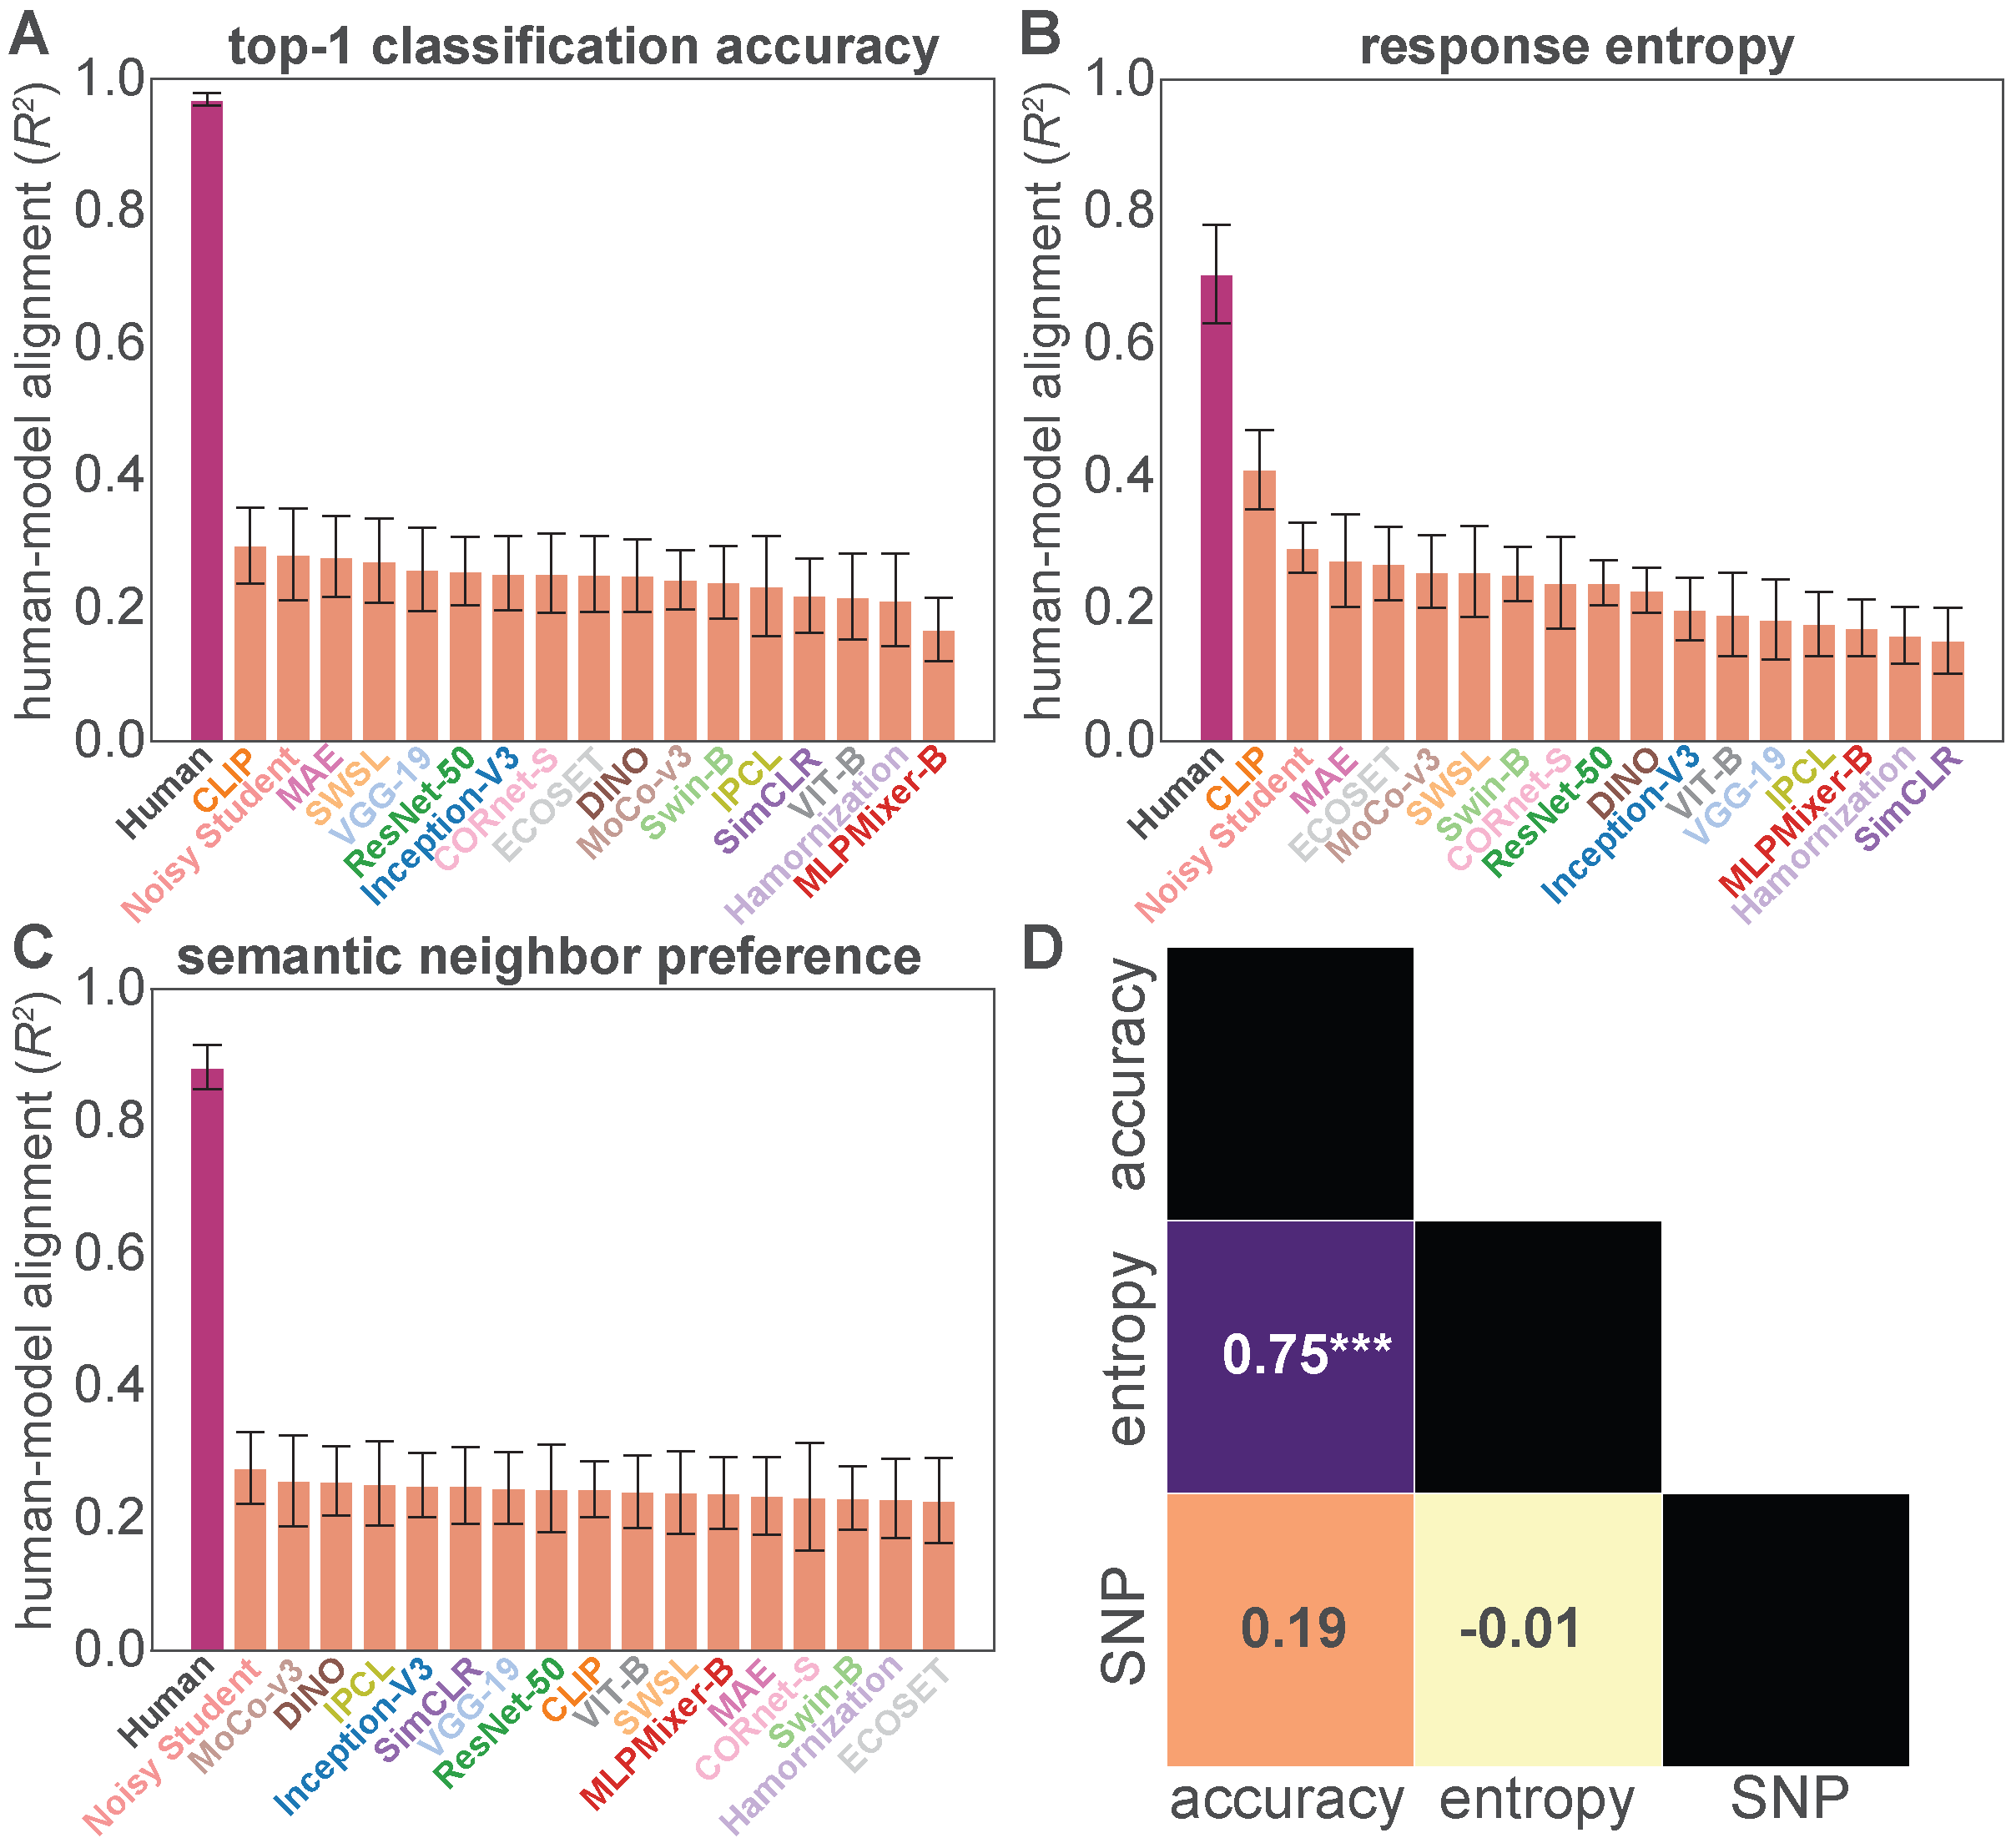
\includegraphics[width=.75\textwidth]{neurips_figures/neurips_reliability_edited_2x2.pdf}
    \caption{Human-model alignment on (A) top-1 classification accuracy, (B) response entropy, and (C) semantic neighbour preference. Leftmost red bars in each plot correspond to baseline human-human consistency on each metric. Error bars indicate bootstrapped 95\% confidence intervals. (D) Spearman $\rho$ correlations between the rank-ordering of vision models with respect to their alignment to human performance on each metric.}
    \label{fig:alignment}
    \vspace{-1em}
\end{figure}
\textbf{A large gap remains between human and model sketch understanding.}
While both humans and models are affected by the amount of detail in sketches, it is not yet clear to what degree their response patterns are well aligned. 
% show similar variations in sketch understanding across levels of detail, are they aligned along these metrics at a more granular level of analysis?
We evaluated human-model alignment scores using the same three metrics (i.e., top-1 classification accuracy, entropy, semantic neighbor preference) by estimating the degree to which model performance on different \textit{types} of sketches (e.g., lions drawn in 4 seconds or less) covaried systematically with human performance on the same \textit{types} of sketches. 
For example, a model is considered well aligned with humans with respect to recognition performance if it achieves high top-1 classification accuracy on the same types of sketches that humans succeed in classifying \textit{and} if it achieves low accuracy on the types of sketches that humans fail to classify. 
Similarly, a model is considered well aligned with humans with respect to semantic ambiguity if it produces a response distribution with high entropy for the same types of sketches that humans are also highly uncertain about \textit{and} if it produces a low-entropy response distribution for the types of sketches that humans systematically agree on (regardless of whether this agreement is concentrated on the correct label).
% \end{wraptable}
% We sought to test how aligned humans and models were on top-1 classification accuracy, response entropy, and semantic neighbor preference for each \textit{kind} of sketch. 
% Here, \textit{kind} refers to sketches of a given concept category at a given level of detail. 
% Our dataset had 128 concepts $\times$ 4 draw duration conditions, furnishing 512 kinds of sketches.
% We fit linear mixed-effects models predicting model performance from human performance along our 3 metrics. We included a fixed-effect interaction term for drawing duration to account for variance across the different levels of sparsity and a fixed-effect term for vision-model type to account for variations in human-model alignment across vision models.
We found that models generaly displayed some degree of alignment to humans on top-1 classification accuracy ($\beta= 7.70\times10^{-2}$, $t=6.77$, $p<.001$), response entropy ($\beta=1.17\times10^{-1}$, $t=28.52$, $p<.001$), and semantic neighbor preference ($\beta = 6.66\times10^{-2}$, $t = 6.21$, $p<.001$). 
Moreover, we found that different vision models aligned with humans to varying degrees (top-1 classification accuracy: $\chi^2(16) = 134.81$, $p<.001$; response entropy: $\chi^2(16) = 725.78$, $p<.001$; semantic neighbor preference: $\chi^2(16) = 5.05$, $p=.99$).
% $\chi^2$ model comparisons between models with and without a fixed-effect term for vision model-type revealed that while there was significant variation across vision models with respect to human-model alignment for top-1 classification accuracy ($\chi^2(16) = 134.81$, $p<.001$) and response entropy ($\chi^2(16) = 725.78$, $p<.001$), all models showed similar alignment for semantic neighbor preference ($\chi^2(16) = 5.05$, $p=.99$).
Nevertheless, a sizable gap remains between the most aligned models and a human-human consistency baseline for \textit{all} metrics (Fig~\ref{fig:alignment}; top-1 classification accuracy: $t = 952.19$, $p<.001$; response entropy: $t = 184.21$, $p<.001$; semantic neighbor preference: $t=389.56$, $p<.001$).
Finally, we observe that while examining classification accuracy and entropy yield similar rankings over which models are best aligned to humans, these metrics appear to capture non-redundant sources of information about human and model sketch understanding (Fig~\ref{fig:alignment}D).


% Welch's t-tests comparing human-human consistency to overall human-model alignment across models revealed a statistically significant difference for top-1 classification accuracy ($t = 952.19$, $p<.001$), response entropy ($t = 184.21$, $p<.001$), and semantic neighbor preference ($t=389.56$, $p<.001$) supporting the notion of notable gap between human-model alignment and a human-human baseline.

% While each of our 3 metrics highlight gaps in alignment, we also note that each metric provides \textit{unique} insight into ways that models can be brought into closer alignment with human behavior, such that efforts can focus on closing the gap on each of these 3 fronts.
% Evidence for this notion can be seen in the fact that each metric provides a sufficiently different ordering of models in terms of alignment. 
% Figure XXX shows a matrix of Spearman $rho$ correlations between the ordering of models according to each metric. 
% We find that no two metrics are perfectly correlated lending support to the idea that each metric captures non-redundant sources of variation in sketch understanding.

% Figure XXX A shows the amount of variance in human recognition accuracy that can be explained as a function of vision model recognition accuracy while accounting for the effect of draw duration and its interaction with vision model accuracy. 
% In general, we show that while not all models were equally aligned with human recognition accuracy (STAT), there remains a sizeable gap between the most well-aligned models and human-human consistency.
% We investigated the alignment between label response entropy values between each vision model and humans to measure the degree to which the degree of uncertainty expressed by humans aligned with that of vision models.
% For humans, we computed the entropy of the normalized label counts and for vision models, we computed the entropy of the classifier class probabilities.
% Figure XXX B shows the amount of variance in human response entropy that can be explained as a function of vision model response entropy while accounting for the effect of draw duration and its interaction with vision model accuracy.
% Similar to recognition accuracy, we find that while there is some variance amongst models, even the most well-aligned models fall short of the human-human consistency baseline.



% First, we fit mixed-effect linear regression models predicting mean human top-1 accuracy from vision model top-1 accuracy and model-type with by-concept random slopes and intercepts to account for variability within concepts.
% We found that model performance was a significant predictor of human recognition performance ( $\beta = 2.96\times10^{-1}$ $SE= 2.36\times 10^{-2}$, $p<.001$). 
% Furthermore, model comparisons revealed a significant effect of model-type for sketches ($\chi(11)=552.92$, $p<.001$), adding additional support to the notion that some vision models are more consistent with human recognition performance than others (Fig. \ref{fig:VAB_polysemy}, \textit{middle}).
% Specifically, these analyses revealed that CLIP explains the greatest amount of variance in human recognition accuracy, while MLP-Mixer explains little variance.
% While there is some discrepancy between which models are more accurate when comparing performance on human sketches vs. CLIPasso sketches, we generally saw that models that have better recognition performance across both datasets (Fig. \ref{fig:VAB_recog}) are also more consistent with human recognition performance. 
% % (\ref{fig:recognition_performance}

% Second, we computed the entropy of the distributions over object labels for each of the 8,192 sketches, using the normalized label counts and classifier class probabilities, respectively (Fig.~\ref{fig:VAB_polysemy}, \textit{right}). 
% Next, we fit mixed-effect models predicting human response entropy from model class probability entropy and model-type with by-concept random slopes and intercepts for entropy. 
% Similar to model comparisons to human recognition accuracy, we found that model entropy significantly predicted human response entropy ($\beta=2.04 \times10^{-1}$, $SE=6.57\times10^{-3}$, $p<.001$). 
% Additionally, model comparisons revealed a significant effect of model-type for sketches ($\chi^2(11) = 1241.30$, $p<.001$) with CLIP again being the most aligned model.
% These evaluations of accuracy and uncertainty reveal that both state-of-the-art model performance and the distributions underlying that performance is predictive of the same constructs for human recognition performance to varying degrees, with some models being more consistent with human behavior than others. 

% \subsection{Benchmarking machine sketch production}

\textbf{A CLIP-based sketch generation algorithm emulates human sketches under some conditions.}

While sketch understanding is a critical aspect of visual abstraction, the ability to \textit{produce} sketches spanning different levels of abstraction is no less important.
Although there remains a gap between human and model sketch understanding, a CLIP-based vision model \cite{radford2021learning} was among the most performant and best aligned to human sketch understanding. 
% our results thus far highlight the promise of CLIP, one of the models that displayed the strongest alignment with human sketch understanding. 
% a large vision-language model trained on web-scale data, CLIP, is among the most performant models at sketch recognition without any fine-tuning and also one of the most well aligned models to human sketch understanding.
Insofar as the major bottleneck to being able to generate more human-like sketches is achieving more human-like understanding of sketches and other images \cite{fan2018common}, a generative model leveraging CLIP's latent representation may be a promising approach. % could a generative model that leverages CLIP's latent features generate sketches at multiple levels of visual abstraction?
Consistent with this possibility, we found that \texttt{CLIPasso} generated sketches of concepts at each abstraction level were about as recognizable as the human-generated sketches of those same concepts at the same abstraction level (Fig.~\ref{fig:CLIPasso-results}A; $adjusted \: R^2 = .64$).
% human sketches of a given concept at a particular abstraction level (e.g., lions drawn in 32s) that were 
% As can be seen in Figure (XXX) human recognition accuracy for human sketches and CLIPasso sketches were comparable at each level of `production budget' (draw duration for human sketches, number of strokes for CLIPasso sketches).
% We fit a mixed-effect linear regression model predicting top-1 classification accuracy of human sketches from top-1 classification accuracy of the same \textit{kind} of CLIPasso sketches with an interaction term for abstraction level (number of strokes).
% Overall, we found a close correspondence between people's recognition performance on human and CLIPasso performance ($adjusted \: R^2 = .64$).
Moreover, we found that the more detailed \texttt{CLIPasso} sketches were especially human-like in that they evoked a similar set of meanings to their human-generated counterparts.
% Since human recognition performance on CLIPasso sketches does not perfectly account for performance on human drawings, this indicates that while humans see \textit{some} similar structure between human-made and CLIPasso-generated sketches of the same concept at each level of abstraction, there are some sketches that lead to diverging human responses depending on whether they are made by humans or CLIPasso. 

To measure the degree to which human and \texttt{CLIPasso} sketches converged with respect to the object labels that they elicited from human viewers, we computed the Jensen-Shannon distance (JSD) between the label distributions of human and \texttt{CLIPasso} sketches for each concept at each of the 4 levels of abstraction.
% We compared the vector of human label responses between CLIPasso and human sketches of each concept at each level of abstraction using the Jensen-Shannon distance (JSD) between the normalized human-generated label counts. 
In Fig. \ref{fig:CLIPasso-results} B. we show the average label divergence at each level of abstraction.
% For each \textit{kind} of CLIPasso sketch, kind referring to sketches of each concept at each of the 4 constraint levels, we ranked each kind of human sketch in terms of their JSDs.
% We computed the minimum rank amongst human sketches of the same concept at each level of constraint for CLIPasso sketches (number of strokes).
% This captures the minimum divergence between the target CLIPasso sketch and \textit{any} human sketch of the same concept regardless of level of abstraction.
% We found that more detailed sketches, i.e., those with a greater number of strokes, tended to have an overall higher rank across concepts.
We found that humans and \texttt{CLIPasso} sketches were least divergent in terms of their perceived meaning when they were depicted in greater detail or were \textit{less abstract} ($\beta = -0.69$, $t=-6.86$, $p<.001$).
At lower levels of detail and visual fidelity, human and \texttt{CLIPasso} sketches elicited more diverging responses.
Thus, while \texttt{CLIPasso} more closely approximates human sketch production behavior at greater levels of detail, there remains a large gap between how \texttt{CLIPasso} and human participants attempted to preserve sketch meaning under more severe production constraints. 
Taken together, while \texttt{CLIPasso} marks significant progress towards human-like sketch production its ability to produce highly abstract sketches in a human-like manner remains limited.

\begin{wrapfigure}{r}{.6\textwidth}
    \centering
    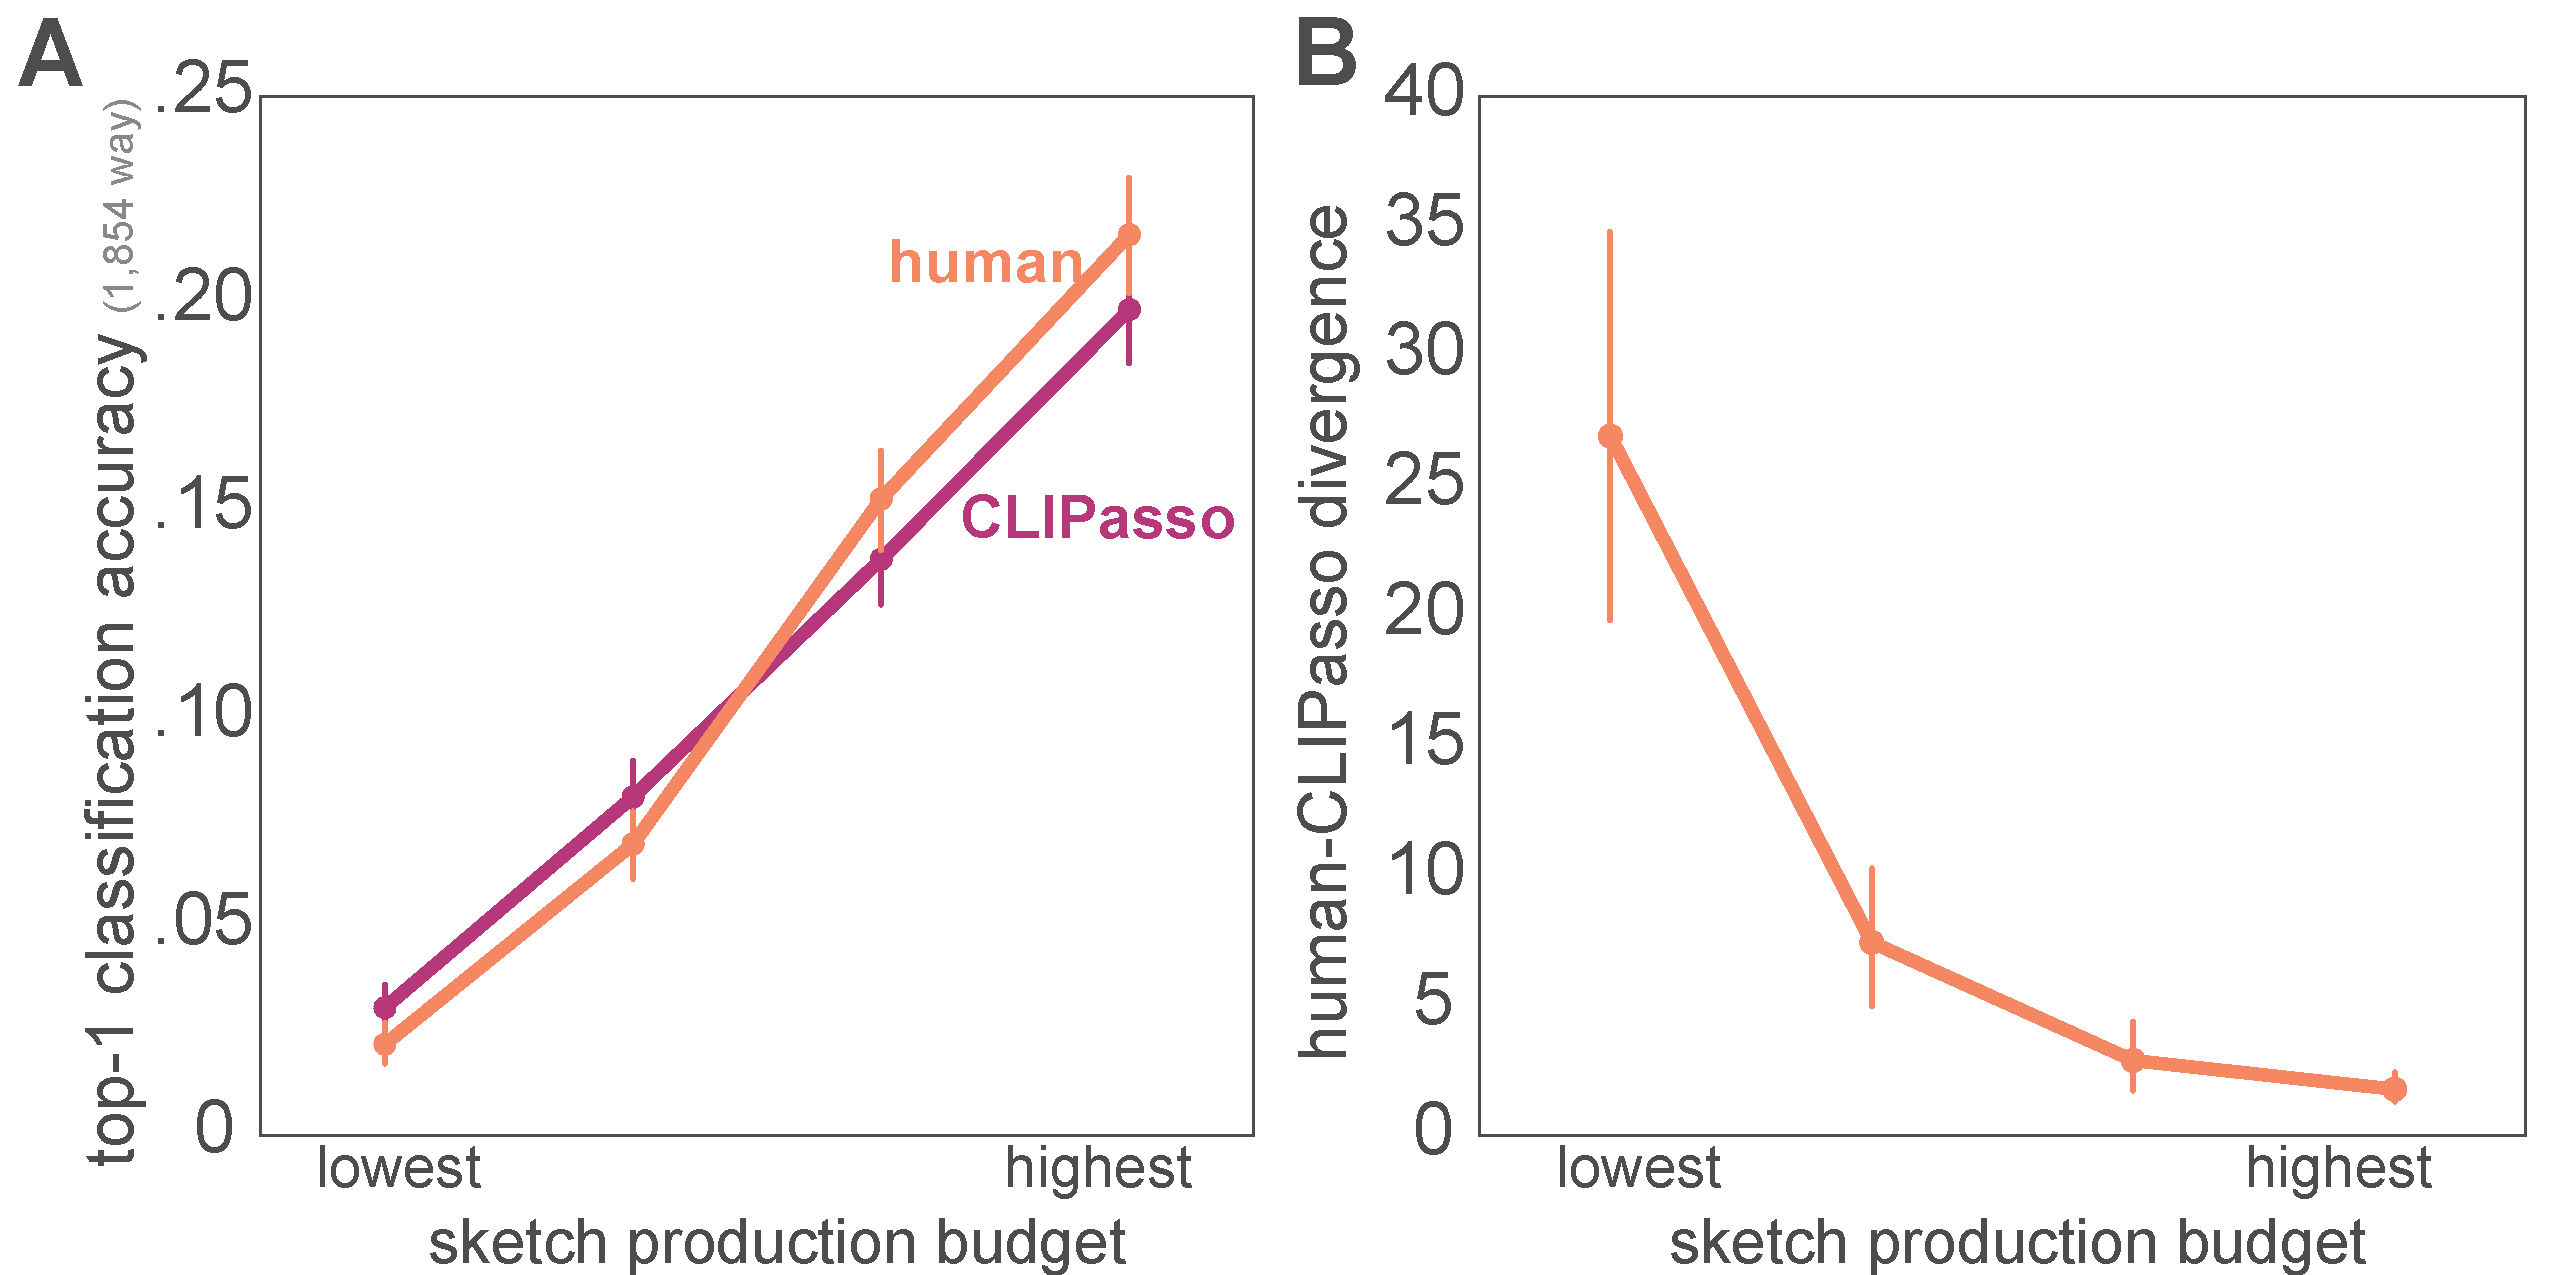
\includegraphics[width=.6\textwidth]{neurips_figures/neurips_CLIPasso_edited.pdf}
    \caption{(A) Human top-1 recognition performance on \texttt{CLIPasso} and human sketches at different production budgets (draw duration for human sketches and number of strokes for \texttt{CLIPasso} sketches). (B) Divergence in human-responses to the same type of human and \texttt{CLIPasso} sketches as a function of sketch production budget.}
    % \vspace{-1em}
    \label{fig:CLIPasso-results}
\end{wrapfigure}

% While vision is one facet of achieving human-like sketch comprehension, how effectively do contemporary generative models leverage semantic information embedded within objects to create abstractions in drawings as humans do?

% To investigate this alignment between human and machine sketch methodology, we fit mixed-effect linear regression models predicting mean human top-1 accuracy from vision model top-1 accuracy and model-type with by-concept random slopes and intercepts to account for variability within concepts. Similar to that displayed by human sketches, we found that model performance was a significant predictor of human recognition performance of machine sketches ($\beta = 2.97\times10^{-1}$, $SE = 2.34 \times 10^{-2}$, $p<.001$). 
% We computed the entropy of the distributions over object labels for each of the 8,192 sketches across the CLIPasso sketch dataset, using the normalized label counts and classifier class probabilities, respectively (Fig.~\ref{fig:VAB_polysemy}, \textit{right}). 
% We then computed the entropy of the distributions over object labels for each of the 8,192 sketches across the CLIPasso sketch dataset, using the normalized label counts and classifier class probabilities, respectively (Fig.~\ref{fig:VAB_polysemy}, \textit{right}). 
% Next, we fit mixed-effect models predicting human response entropy from model class probability entropy and model-type with by-concept random slopes and intercepts for entropy. Similar to model comparisons to human recognition accuracy, we found that model entropy significantly predicted human response entropy ($\beta_{machine \; sketches} = 2.09 \times10^{-1}$, $SE = 7.90 \times10^{-3}$, $p<.001$)

% Additionally, model comparisons revealed a significant effect of model-type for machine ($\chi^2(11) = 1509.00$, $p<.001$) sketches, although CLIP was found to be the highest performing model for both human and CLIPasso sketches when using this metric.

% To evaluate whether machine sketches also display recognition uncertainty at varying degrees of abstraction, we also compared an intercept-only model to a model with a factor for number of strokes and found a significant effect of number of strokes ($F (3,260) = 3.19$, $p < .05$). Thus, for machine generated sketches, there did appear to be an effect of stroke number on the consistency between models in their expressed semantic uncertainty with models being less consistent in their classifications of sketches with more strokes.

% These evaluations of accuracy and uncertainty in machine generated sketches reveal that both vision and human performance is similar to that of human sketches across a range of abstraction levels.

%For sketches generated using CLIPasso, we also compared an intercept-only model to a model with a factor for number of strokes and found a significant effect of number of strokes ($F (3,260) = 3.19$, $p < .05$). Thus, for machine generated sketches, there did appear to be an effect of stroke number on the consistency between models in their expressed semantic uncertainty with models being less consistent in their classifications of sketches with more strokes. 

%First, we fit mixed-effect linear regression models predicting mean human top-1 accuracy from vision model top-1 accuracy and model-type with by-concept random slopes and intercepts to account for variability within concepts.We found that model performance was a significant predictor of human recognition performance ($\beta_{machine \; sketches}= 2.97\times10^{-1}$, $SE = 2.34 \times 10^{-2}$, $p<.001$). Furthermore, model comparisons revealed a significant effect of model-type for machine sketches ($\chi(11)=741.51$, $p<.001$), adding additional support that some vision models are more consistent with human recognition performance than others (Fig. \ref{fig:VAB_polysemy}, \textit{middle}).

%Second, we computed the entropy of the distributions over object labels for each of the 8,192 sketches across the CLIPasso sketch dataset, using the normalized label counts and classifier class probabilities, respectively (Fig.~\ref{fig:VAB_polysemy}, \textit{right}).  

%Next, we fit mixed-effect models predicting human response entropy from model class probability entropy and model-type with by-concept random slopes and intercepts for entropy. Similar to model comparisons to human recognition accuracy, we found that model entropy significantly predicted human response entropy ($\beta_{machine \; sketches} = 2.09 \times10^{-1}$, $SE = 7.90 \times10^{-3}$, $p<.001$)

%Additionally, model comparisons revealed a significant effect of model-type for machine ($\chi^2(11) = 1509.00$, $p<.001$) sketches, although CLIP was found to be the highest performing model for both human and CLIPasso sketches when using this metric.
% \vspace{-3 em}
% \vspace{-1em}
\newpage
\section{Conclusion}
\vspace{-1 em}
Recent advances in machine vision have enabled new opportunities to understand the computational mechanisms that underlie human-like visual abstraction---how humans create and interpret a wide variety of images (from detailed illustrations to schematic diagrams) to convey what they perceive and know about the world. 
% There has been incredible progress in recent years in the development of high performing vision models, which have steadily achieved enough variation in model architecture and training to prime cognitive psychology research with the opportunity to begin explore the extent to which specific models have achieved human-like understanding of abstract symbolic representations, like sketches.
Here we introduce \texttt{SEVA}, a new dataset and benchmark containing approximately 90K human and machine generated sketches spanning multiple levels of abstraction, to evaluate progress towards alignment between human and machine visual abstraction. 
 % Critically, our dataset is the first sketch dataset to include systematic variation in sparsity in order to test state-of-the-art vision models in their ability to achieve human-like understanding of visual concepts across multiple levels of abstraction. 
Critically, our model evaluation protocol is focused not just on performance but on how well these models approximate \textit{human-like} sketch production and understanding.
Initial benchmarking of a set of 17 vision models on \texttt{SEVA} following this protocol revealed that even the most performant and well-aligned models deviate from human behavior in systematic ways.
We also find that current generative models of sketching are able to sketch in human-like ways, but only in limited settings. 

We hope that \texttt{SEVA} will accelerate progress towards unified computational theories that explain how humans are capable of generating and understanding such a wide variety of abstract visual representations.
Specifically, our dataset could be used to adjudicate between vision models that are high-performing on tasks involving natural images \cite{mahmoud2023stress,golan2020controversial} by characterizing their alignment with how humans understand images generated in a very different manner, including freehand sketches. 
In addition, \texttt{SEVA} is distinctive among existing human sketch datasets in that it contains detailed measurements of how humans make moment-to-moment decisions about where to place each stroke, when aiming to produce a sketch of a visible object, under different constraints. 
As such, we expect \texttt{SEVA} to be a key resource for advancing the state-of-the-art in sketch generation \cite{qiu2022emergent,wang2021sketchembednet, vinker2022clipasso,ha2017neural,ribeiro2020sketchformer}, and thus lead to computational models of generalized visual abstraction. 

\vspace{-1em}
\section{Limitations}
\vspace{-1em}
We note several limitations of the current study that would be important to address in future work. 
\underline{First}, our sample of participants was limited to English-speaking individuals based in the United States. As such, the current study cannot speak to potential differences in sketch-production behavior across geographical and cultural contexts. 
However, future work that recruits from a broader cross-section of individuals, including those located in the ``Majority World,'' will be vital for understanding those potential sources of variation in human sketch production and comprehension. 
\underline{Second}, we recruited participants via Prolific, a widely used crowdsourcing platform in human behavioral research, without regard to any previous artistic training they had received. As such, our study generally reflects sketch production behavior among individuals without substantial expertise in the visual arts.
\underline{Third}, following prior work \cite{fan2018common, fan2020pragmatic, hawkins2023visual,yu2016sketch,jongejan2017quick, long2021parallel}, the human sketches in our dataset were obtained using a web-based digital drawing interface, where most participants used a mouse or trackpad to produce their sketches (89.96\%) and some participants used a touchscreen (6.94\%) or a stylus (1.67\%). 
Investigation of the impact of input device on sketch production would be a fruitful avenue for follow-up work. 
\underline{Fourth}, because we did not obtain non-digital sketches (e.g., drawn on paper with a pen/pencil), our data cannot speak to differences between digital and non-digital sketches.
\underline{Fifth}, our study of machine sketch production included just one model, \textit{CLIPasso}, limiting the conclusions that can be drawn about sketch generation algorithms in general. Future work that evaluates a broader suite of algorithms would thus be valuable. 

% \kushin{While we believe that all data collection in service of constructing \texttt{SEVA} was done in a rigorous manner, we note that our data collection was limited to Prolific participants residing in the United States. 
% It has been well documented how restricting data collection to  western, educated, industrialized, rich and democratic (WEIRD) societies has skewed psychological research \cite{henrich2010most} and it is possible that the sketches of our various concepts might systematically vary between the US and other populations.
% Each participant in our drawing studies only made drawings under one of the four possible time constraint conditions (4s, 8s, 16s, 32s). 
% While this was done so that participants' experience of drawing a concept under one time-constraint wouldn't affect their drawing of the concept under a different constraint, it is possible that this introduced greater variance in our dataset.
% While an abundance of studies have validated the use of online digital drawing platforms for collecting human sketch data 
% \cite{fan2018common, fan2020pragmatic, hawkins2023visual,yu2016sketch,jongejan2017quick, long2021parallel}, it remains true that people might have less experience drawing with a mouse than with a drawing tool such as a pen or pencil. 
% The vast majority of sketches in \texttt{SEVA} were made using either a mouse or trackpad (89.9\%) with a small minority made using either touch-screens (6.94\%) or styluses (1.67\%).
% Additionally, while we borrow the time-constrained drawing task from \cite{berger2013style}, the original study was conducted using a sample of trained artists, while our study was conducted using a sample of non-experts on Prolific.
% Since our goal was to study visual abstraction as a general phenomenon, we believe that the expertise of our participant pool should not affect our conclusions.}


% , as well as help explain how we are able to invent symbolic systems for encoding abstract knowledge in pictorial form.
% Progress along these lines will lead to more human-aligned models of vision that can flexibly recognize visual concepts as well as depict them in human-like ways.


% We also found that models generally agree in their expressed uncertainty over object classes when recognizing sketches and that this uncertainty remains largely consistent across varying levels of abstraction and detail, but with models being less consistent across abstraction levels over their uncertainty in machine generated sketches.
% This points to an intriguing yet critical gap in the fidelity of sketch production algorithms to human sketch behavior, and we hope results such as ours will help open avenues for closing this gap in human-machine sketch production.

% % Yael: Maybe what I wrote below could serve as a Conclusion, summarizing how this benchmark can be used to test the "human-like" abilities of these super strong models.


% Recently, there has been a huge acceleration in the development of image generation algorithms, with new models introducing unprecedented high quality results for extremely challenging tasks such as text-to-image generation, image-to-image generation, image editing, and more. This raises the intriguing question of whether these models can simulate human understanding and creativity.

% We hope our benchmark could assist with evaluating the abilities of future models in performing complicated tasks such as generation and reasoning of abstract sketches.

% % the general idea for this section is to highlight other generative models and how our efforts relate to them! I’m sure you’re more than used to highlighting the distinctions between approaches like CLIPasso and diffusion models etc., but it might be worth really emphasizing that here in light of what we find!
% XXXX

% There has been incredible progress in the development of high performing vision models over the past several years--and recently, reaching enough variation in model architecture and training to prime cognitive psychology research with the opportunity to begin explore the extent to which specific models have achieved human-like understanding of abstract symbolic representations, like sketches.
% To evaluate this expansive range of state-of-the-art vision models and their ability to extract meaning from sketch representations, we introduce a new large-scale drawing dataset of approximately 90K sketches based on 2,048 real-world objects spanning 128 diverse concept categories.
% Our dataset combines both human-made and AI-generated sketches produced under varying production constraints (limitations in drawing duration for human sketchers, and limitations in number of strokes for CLIPasso \cite{vinker2022clipasso}). 
% By systematically varying the level of abstraction produced by these different production constraints, our dataset provides a rich testbed to investigate human and machine visual understanding of human and machine sketches. 

% In an era where it is becoming increasingly difficult to adjudicate between state-of-the-art vision models in terms of their relevance to human cognition, our dataset provides a novel substrate to tease apart which models are more human-like than others \cite{golan2020controversial}.
% We provide initial benchmarking of a representative set of vision models spanning architectures and training techniques against human generated soft-label distributions for a representative set of sketches from both datasets. 
% Across a battery of model evaluations, we broadly find that the models that we investigated are sensitive to the variation in the semantic information produced by different production constraints and that some models, like CLIP, are more consistent with human recognition of sketches than others, like MLP-Mixer. 
% We also found that models generally agree in their expressed uncertainty over object classes when recognizing sketches and that this uncertainty remains largely consistent across varying levels of abstraction and detail, but with models being less consistent across abstraction levels over their uncertainty in machine generated sketches.
% This points to an intriguing yet critical gap in the fidelity of sketch production algorithms to human sketch behavior, and we hope results such as ours will help open avenues for closing this gap in human-machine sketch production.


% Within our present work, we offer object concept classification as an initial benchmarking protocol to evaluate different models.
% However, we predict future work will seek to benchmark a wider variety of models including those inspired by cognitive neuroscience \cite{chen2022unsupervised, zhuang2021unsupervised,kubilius2019brain} and will seek to build more robust metrics of abstraction beyond those tied to classification-based accuracy.

% Our work complements ongoing efforts to understand how different components of current AI vision models give rise to their classification behavior \cite{hermann2020shapes, nguyen2020wide,schott2021visual,chen2021intriguing} and where limitations might arise in mapping model performance to human cognition \cite{ zhou2019humans,bowers2022deep, mahowald2023dissociating}. 
% In the long run, progress along these research fronts may shed light upon the computational basis of humans' ability to produce highly abstract but nonetheless meaningful representations, as well as invented symbolic systems for encoding abstract knowledge in pictorial form.
% \cite{schmandt2010writing, chrisomalis2020reckonings}.
\newpage
\section*{Acknowledgements}
\textit{Blinded for review.}
\section*{Broader Impacts}

Visual abstraction is as ubiquitous as it is central to our understanding of the visual world.
Humans can recognize depictions of objects at varying levels of fidelity to their real-world counterparts. 
This ability to recognize and render concepts in abstract forms is crucial for visual knowledge transmission in the form of graphs, diagrams, and symbols.
While computer vision has steadily made progress towards algorithms that can recognize objects in scenes, distinguish among different instances of an object, or even answer questions about those objects in natural language, it remains unclear if these systems have the capability to understand visual concepts at multiple levels of abstraction in a human-like manner.
\texttt{SEVA} marks a step towards evaluating current vision algorithms on their sensitivity to depictions of a wide variety of common object concepts at varying levels of abstraction.
Critically, we also provide results on \textit{human} performance on sketch understanding for sketches of varying sparsity, setting a clear benchmark for future vision algorithms.
Our initial study of state-of-the-art vision algorithms shows that even the most high-performing of models still fall short of human consistency baselines.
With these vision algorithms increasingly being deployed in many aspects of everyday life, it is crucial to measure how human-like they are in this most natural of human abilities. 
We hope that \texttt{SEVA} will be used by the community to help close the gaps in current vision algorithms' alignment to human behavior that we have identified in this paper.
% Visual abstraction is a powerful tool that enables humans to distill complex information, ranging from diagrams and flowcharts to the diverse symbols found in city highways, into a simplified and accessible form.
% Despite extensive progress on algorithmic understanding and creation of images and scenes, the capacity of these models to effectively grasp varying levels of visual abstraction remains an open question in many AI applications, including the creation of graphics and logos, data visualization and infographics, user interface design, visual storytelling and animation, and other fields that require condensing information into visual forms. As such, we believe the SEVA benchmark is a key step toward measuring whether a given algorithm is sensitive to visual abstraction akin to human capabilities. In the case that sensitivity to visual abstraction becomes a crucial aspect of achieving high performance in some real-world domain, SEVA (or its successors) could be used to screen for algorithms more likely to generalize to a wide range of visual representations. Furthermore, our results, while representative of only an initial survey of existing algorithms, do suggest that models with a symbolic understanding of the world (e.g. CLIP-ViT) better mirror human comprehension of visual abstraction, suggesting that symbolic representations may be key to human-like inferences about visual abstraction for vision algorithms.

\bibliography{references}{}
\bibliographystyle{plain}

% \subsection{Style}


% Papers to be submitted to NeurIPS 2022 must be prepared according to the
% instructions presented here. Papers may only be up to {\bf nine} pages long,
% including figures. Additional pages \emph{containing only acknowledgments and
% references} are allowed. Papers that exceed the page limit will not be
% reviewed, or in any other way considered for presentation at the conference.


% The margins in 2022 are the same as those in 2007, which allow for $\sim$$15\%$
% more words in the paper compared to earlier years.


% Authors are required to use the NeurIPS \LaTeX{} style files obtainable at the
% NeurIPS website as indicated below. Please make sure you use the current files
% and not previous versions. Tweaking the style files may be grounds for
% rejection.


% \subsection{Retrieval of style files}


% The style files for NeurIPS and other conference information are available on
% the World Wide Web at
% \begin{center}
%   \url{http://www.neurips.cc/}
% \end{center}
% The file \verb+neurips_2022.pdf+ contains these instructions and illustrates the
% various formatting requirements your NeurIPS paper must satisfy.


% The only supported style file for NeurIPS 2022 is \verb+neurips_2022.sty+,
% rewritten for \LaTeXe{}.  \textbf{Previous style files for \LaTeX{} 2.09,
%   Microsoft Word, and RTF are no longer supported!}


% The \LaTeX{} style file contains three optional arguments: \verb+final+, which
% creates a camera-ready copy, \verb+preprint+, which creates a preprint for
% submission to, e.g., arXiv, and \verb+nonatbib+, which will not load the
% \verb+natbib+ package for you in case of package clash.


% \paragraph{Preprint option}
% If you wish to post a preprint of your work online, e.g., on arXiv, using the
% NeurIPS style, please use the \verb+preprint+ option. This will create a
% nonanonymized version of your work with the text ``Preprint. Work in progress.''
% in the footer. This version may be distributed as you see fit. Please \textbf{do
%   not} use the \verb+final+ option, which should \textbf{only} be used for
% papers accepted to NeurIPS.


% At submission time, please omit the \verb+final+ and \verb+preprint+
% options. This will anonymize your submission and add line numbers to aid
% review. Please do \emph{not} refer to these line numbers in your paper as they
% will be removed during generation of camera-ready copies.


% The file \verb+neurips_2022.tex+ may be used as a ``shell'' for writing your
% paper. All you have to do is replace the author, title, abstract, and text of
% the paper with your own.


% The formatting instructions contained in these style files are summarized in
% Sections \ref{gen_inst}, \ref{headings}, and \ref{others} below.


% \section{General formatting instructions}
% \label{gen_inst}


% The text must be confined within a rectangle 5.5~inches (33~picas) wide and
% 9~inches (54~picas) long. The left margin is 1.5~inch (9~picas).  Use 10~point
% type with a vertical spacing (leading) of 11~points.  Times New Roman is the
% preferred typeface throughout, and will be selected for you by default.
% Paragraphs are separated by \nicefrac{1}{2}~line space (5.5 points), with no
% indentation.


% The paper title should be 17~point, initial caps/lower case, bold, centered
% between two horizontal rules. The top rule should be 4~points thick and the
% bottom rule should be 1~point thick. Allow \nicefrac{1}{4}~inch space above and
% below the title to rules. All pages should start at 1~inch (6~picas) from the
% top of the page.


% For the final version, authors' names are set in boldface, and each name is
% centered above the corresponding address. The lead author's name is to be listed
% first (left-most), and the co-authors' names (if different address) are set to
% follow. If there is only one co-author, list both author and co-author side by
% side.


% Please pay special attention to the instructions in Section \ref{others}
% regarding figures, tables, acknowledgments, and references.


% \section{Headings: first level}
% \label{headings}


% All headings should be lower case (except for first word and proper nouns),
% flush left, and bold.


% First-level headings should be in 12-point type.


% \subsection{Headings: second level}


% Second-level headings should be in 10-point type.


% \subsubsection{Headings: third level}


% Third-level headings should be in 10-point type.


% \paragraph{Paragraphs}


% There is also a \verb+\paragraph+ command available, which sets the heading in
% bold, flush left, and inline with the text, with the heading followed by 1\,em
% of space.


% \section{Citations, figures, tables, references}
% \label{others}


% These instructions apply to everyone.


% \subsection{Citations within the text}


% The \verb+natbib+ package will be loaded for you by default.  Citations may be
% author/year or numeric, as long as you maintain internal consistency.  As to the
% format of the references themselves, any style is acceptable as long as it is
% used consistently.


% The documentation for \verb+natbib+ may be found at
% \begin{center}
%   \url{http://mirrors.ctan.org/macros/latex/contrib/natbib/natnotes.pdf}
% \end{center}
% Of note is the command \verb+\citet+, which produces citations appropriate for
% use in inline text.  For example,
% \begin{verbatim}
%    \citet{hasselmo} investigated\dots
% \end{verbatim}
% produces
% \begin{quote}
%   Hasselmo, et al.\ (1995) investigated\dots
% \end{quote}


% If you wish to load the \verb+natbib+ package with options, you may add the
% following before loading the \verb+neurips_2022+ package:
% \begin{verbatim}
%    \PassOptionsToPackage{options}{natbib}
% \end{verbatim}


% If \verb+natbib+ clashes with another package you load, you can add the optional
% argument \verb+nonatbib+ when loading the style file:
% \begin{verbatim}
%    \usepackage[nonatbib]{neurips_2022}
% \end{verbatim}


% As submission is double blind, refer to your own published work in the third
% person. That is, use ``In the previous work of Jones et al.\ [4],'' not ``In our
% previous work [4].'' If you cite your other papers that are not widely available
% (e.g., a journal paper under review), use anonymous author names in the
% citation, e.g., an author of the form ``A.\ Anonymous.''


% \subsection{Footnotes}


% Footnotes should be used sparingly.  If you do require a footnote, indicate
% footnotes with a number\footnote{Sample of the first footnote.} in the
% text. Place the footnotes at the bottom of the page on which they appear.
% Precede the footnote with a horizontal rule of 2~inches (12~picas).


% Note that footnotes are properly typeset \emph{after} punctuation
% marks.\footnote{As in this example.}


% \subsection{Figures}


% \begin{figure}
%   \centering
%   \fbox{\rule[-.5cm]{0cm}{4cm} \rule[-.5cm]{4cm}{0cm}}
%   \caption{Sample figure caption.}
% \end{figure}


% All artwork must be neat, clean, and legible. Lines should be dark enough for
% purposes of reproduction. The figure number and caption always appear after the
% figure. Place one line space before the figure caption and one line space after
% the figure. The figure caption should be lower case (except for first word and
% proper nouns); figures are numbered consecutively.


% You may use color figures.  However, it is best for the figure captions and the
% paper body to be legible if the paper is printed in either black/white or in
% color.


% \subsection{Tables}


% All tables must be centered, neat, clean and legible.  The table number and
% title always appear before the table.  See Table~\ref{sample-table}.


% Place one line space before the table title, one line space after the
% table title, and one line space after the table. The table title must
% be lower case (except for first word and proper nouns); tables are
% numbered consecutively.


% Note that publication-quality tables \emph{do not contain vertical rules.} We
% strongly suggest the use of the \verb+booktabs+ package, which allows for
% typesetting high-quality, professional tables:
% \begin{center}
%   \url{https://www.ctan.org/pkg/booktabs}
% \end{center}
% This package was used to typeset Table~\ref{sample-table}.


% \begin{table}
%   \caption{Sample table title}
%   \label{sample-table}
%   \centering
%   \begin{tabular}{lll}
%     \toprule
%     \multicolumn{2}{Part}                   \\
%     \cmidrule(r){1-2}
%     Name     & Description     & Size ($\mu$m) \\
%     \midrule
%     Dendrite & Input terminal  & $\sim$100     \\
%     Axon     & Output terminal & $\sim$10      \\
%     Soma     & Cell body       & up to $10^6$  \\
%     \bottomrule
%   \end{tabular}
% \end{table}


% \section{Final instructions}


% Do not change any aspects of the formatting parameters in the style files.  In
% fit into, and do not change font sizes (except perhaps in the
% \textbf{References} section; see below). Please note that pages should be
% numbered.


% \section{Preparing PDF files}


% Please prepare submission files with paper size ``US Letter,'' and not, for
% example, ``A4.''


% Fonts were the main cause of problems in the past years. Your PDF file must only
% contain Type 1 or Embedded TrueType fonts. Here are a few instructions to
% achieve this.


% \begin{itemize}


% \item You should directly generate PDF files using \verb+pdflatex+.


% \item You can check which fonts a PDF files uses.  In Acrobat Reader, select the
%   menu Files$>$Document Properties$>$Fonts and select Show All Fonts. You can
%   also use the program \verb+pdffonts+ which comes with \verb+xpdf+ and is
%   available out-of-the-box on most Linux machines.


% \item The IEEE has recommendations for generating PDF files whose fonts are also
%   acceptable for NeurIPS. Please see
%   \url{http://www.emfield.org/icuwb2010/downloads/IEEE-PDF-SpecV32.pdf}


% \item \verb+xfig+ "patterned" shapes are implemented with bitmap fonts.  Use
%   "solid" shapes instead.


% \item The \verb+\bbold+ package almost always uses bitmap fonts.  You should use
%   the equivalent AMS Fonts:
% \begin{verbatim}
%    \usepackage{amsfonts}
% \end{verbatim}
% followed by, e.g., \verb+\mathbb{R}+, \verb+\mathbb{N}+, or \verb+\mathbb{C}+
% for $\mathbb{R}$, $\mathbb{N}$ or $\mathbb{C}$.  You can also use the following
% workaround for reals, natural and complex:
% \begin{verbatim}
%    \newcommand{\RR}{I\!\!R} %real numbers
%    \newcommand{\Nat}{I\!\!N} %natural numbers
%    \newcommand{\CC}{I\!\!\!\!C} %complex numbers
% \end{verbatim}
% Note that \verb+amsfonts+ is automatically loaded by the \verb+amssymb+ package.


% \end{itemize}


% If your file contains type 3 fonts or non embedded TrueType fonts, we will ask
% you to fix it.


% \subsection{Margins in \LaTeX{}}


% Most of the margin problems come from figures positioned by hand using
% \verb+\special+ or other commands. We suggest using the command
% \verb+\includegraphics+ from the \verb+graphicx+ package. Always specify the
% figure width as a multiple of the line width as in the example below:
% \begin{verbatim}
%    \usepackage[pdftex]{graphicx} ...
%    \includegraphics[width=0.8\linewidth]{myfile.pdf}
% \end{verbatim}
% See Section 4.4 in the graphics bundle documentation
% (\url{http://mirrors.ctan.org/macros/latex/required/graphics/grfguide.pdf})


% A number of width problems arise when \LaTeX{} cannot properly hyphenate a
% line. Please give LaTeX hyphenation hints using the \verb+\-+ command when
% necessary.


% \begin{ack}
% Use unnumbered first level headings for the acknowledgments. All acknowledgments
% go at the end of the paper before the list of references. Moreover, you are required to declare
% funding (financial activities supporting the submitted work) and competing interests (related financial activities outside the submitted work).
% More information about this disclosure can be found at: \url{https://neurips.cc/Conferences/2022/PaperInformation/FundingDisclosure}.


% Do {\bf not} include this section in the anonymized submission, only in the final paper. You can use the \texttt{ack} environment provided in the style file to autmoatically hide this section in the anonymized submission.
% \end{ack}


% \section*{References}


% References follow the acknowledgments. Use unnumbered first-level heading for
% the references. Any choice of citation style is acceptable as long as you are
% consistent. It is permissible to reduce the font size to \verb+small+ (9 point)
% when listing the references.
% Note that the Reference section does not count towards the page limit.
% \medskip


% {
% \small


% [1] Alexander, J.A.\ \& Mozer, M.C.\ (1995) Template-based algorithms for
% connectionist rule extraction. In G.\ Tesauro, D.S.\ Touretzky and T.K.\ Leen
% (eds.), {\it Advances in Neural Information Processing Systems 7},
% pp.\ 609--616. Cambridge, MA: MIT Press.


% [2] Bower, J.M.\ \& Beeman, D.\ (1995) {\it The Book of GENESIS: Exploring
%   Realistic Neural Models with the GEneral NEural SImulation System.}  New York:
% TELOS/Springer--Verlag.


% [3] Hasselmo, M.E., Schnell, E.\ \& Barkai, E.\ (1995) Dynamics of learning and
% recall at excitatory recurrent synapses and cholinergic modulation in rat
% hippocampal region CA3. {\it Journal of Neuroscience} {\bf 15}(7):5249-5262.
% }


% %%%%%%%%%%%%%%%%%%%%%%%%%%%%%%%%%%%%%%%%%%%%%%%%%%%%%%%%%%%%
% \section*{Checklist}


% %%% BEGIN INSTRUCTIONS %%%
% The checklist follows the references.  Please
% read the checklist guidelines carefully for information on how to answer these
% questions.  For each question, change the default \answerTODO{} to \answerYes{},
% \answerNo{}, or \answerNA{}.  You are strongly encouraged to include a {\bf
% justification to your answer}, either by referencing the appropriate section of
% your paper or providing a brief inline description.  For example:
% \begin{itemize}
%   \item Did you include the license to the code and datasets? \answerYes{See Section~\ref{gen_inst}.}
%   \item Did you include the license to the code and datasets? \answerNo{The code and the data are proprietary.}
%   \item Did you include the license to the code and datasets? \answerNA{}
% \end{itemize}
% Please do not modify the questions and only use the provided macros for your
% answers.  Note that the Checklist section does not count towards the page
% limit.  In your paper, please delete this instructions block and only keep the
% Checklist section heading above along with the questions/answers below.
% %%% END INSTRUCTIONS %%%


% \begin{enumerate}


% \item For all authors...
% \begin{enumerate}
%   \item Do the main claims made in the abstract and introduction accurately reflect the paper's contributions and scope?
%     \answerTODO{}
%   \item Did you describe the limitations of your work?
%     \answerTODO{}
%   \item Did you discuss any potential negative societal impacts of your work?
%     \answerTODO{}
%   \item Have you read the ethics review guidelines and ensured that your paper conforms to them?
%     \answerTODO{}
% \end{enumerate}


% \item If you are including theoretical results...
% \begin{enumerate}
%   \item Did you state the full set of assumptions of all theoretical results?
%     \answerTODO{}
%         \item Did you include complete proofs of all theoretical results?
%     \answerTODO{}
% \end{enumerate}


% \item If you ran experiments...
% \begin{enumerate}
%   \item Did you include the code, data, and instructions needed to reproduce the main experimental results (either in the supplemental material or as a URL)?
%     \answerTODO{}
%   \item Did you specify all the training details (e.g., data splits, hyperparameters, how they were chosen)?
%     \answerTODO{}
%         \item Did you report error bars (e.g., with respect to the random seed after running experiments multiple times)?
%     \answerTODO{}
%         \item Did you include the total amount of compute and the type of resources used (e.g., type of GPUs, internal cluster, or cloud provider)?
%     \answerTODO{}
% \end{enumerate}


% \item If you are using existing assets (e.g., code, data, models) or curating/releasing new assets...
% \begin{enumerate}
%   \item If your work uses existing assets, did you cite the creators?
%     \answerTODO{}
%   \item Did you mention the license of the assets?
%     \answerTODO{}
%   \item Did you include any new assets either in the supplemental material or as a URL?
%     \answerTODO{}
%   \item Did you discuss whether and how consent was obtained from people whose data you're using/curating?
%     \answerTODO{}
%   \item Did you discuss whether the data you are using/curating contains personally identifiable information or offensive content?
%     \answerTODO{}
% \end{enumerate}


% \item If you used crowdsourcing or conducted research with human subjects...
% \begin{enumerate}
%   \item Did you include the full text of instructions given to participants and screenshots, if applicable?
%     \answerTODO{}
%   \item Did you describe any potential participant risks, with links to Institutional Review Board (IRB) approvals, if applicable?
%     \answerTODO{}
%   \item Did you include the estimated hourly wage paid to participants and the total amount spent on participant compensation?
%     \answerTODO{}
% \end{enumerate}


% \end{enumerate}


% %%%%%%%%%%%%%%%%%%%%%%%%%%%%%%%%%%%%%%%%%%%%%%%%%%%%%%%%%%%%

\newpage
\appendix


\section{Appendix}

\subsection{Paper Checklist}

\textbf{Do the main claims made in the abstract and introduction accurately reflect the paper's contributions and scope?}
Yes, we provide titled subsections in the Results section that address the questions we raise and claims we posit with experimental results.

\textbf{Have you read the ethics review guidelines and ensured that your paper conforms to them?}

Yes.

\textbf{ Did you discuss any potential negative societal impacts of your work?}

No. We believe our dataset and work is largely benign and that it would be extremely difficult to leverage it for harmful purposes and that the results and data by themselves do not constitute any threat.

\textbf{ Did you describe the limitations of your work?}

We leverage the \texttt{SEVA} dataset that we collected her eto highlight limitations of state-of-the art vision models.
We do not propose novel algorithms ourselves.
We mention in the Introduction how sketching is one \textit{form} of many kinds of visual abstraction including graphs, diagrams, etc.

\textbf{
 Did you include the code, data, and instructions needed to reproduce the main experimental results (either in the supplemental material or as a URL)?}

 Yes, we will make our results available via a public GitHub repository and make our dataset accessible on S3.


\textbf{ Did you specify all the training details (e.g., data splits, hyperparameters, how they were chosen)?}

We did not train or finetune models but did evaluate a suite of pretrained models. We specify details in our Evaluation Protocol section

\textbf{Did you report error bars (e.g., with respect to the random seed after running experiments multiple times)}?

We do present error bars for all our results. These error bars are either analytically computed based on our data as they are or by bootstrapping samples from our dataset. 
We also performance statistical tests to support our results

\textbf{
Did you include the amount of compute and the type of resources used (e.g., type of GPUs, internal cluster, or cloud provider)?}

No, we did not run any highly compute intesive processes. We run all our analyses on personal machines and some model evaluations on internal clusters.

\textbf{ Did you mention the license of the assets?}

In our datasheet we mention that we plan to release our dataset under an MIT license.

\textbf{Did you include any new assets either in the supplemental material or as a URL?}

Yes, we plan to publicly release the dataset associated with this paper.

\textbf{ Did you discuss whether and how consent was obtained from people whose data you're using/curating?}

Yes, participants in our studies provided informed consent in accordance with the UCSD IRB.

\textbf{Did you discuss whether the data you are using/curating contains personally identifiable information or offensive content?}

No. Our dataset only contains Prolific worker IDs and information about which US state the participants performed the online study in. 
We do not use or share this information.

\textbf{Did you include the full text of instructions given to participants and screenshots, if applicable?}

No, but we can include this information in supplemental material if it is deemed to be useful to the community by reviewers.
We include details regarding their compensation and the tasks they performed in detail in our Methods section.

\textbf{ Did you describe any potential participant risks, with links to Institutional Review Board (IRB) approvals, if applicable?}

No, but participants were informed about potential study risks (if there were any) along with links to the UCSD when they participated in our tasks.

\textbf{Did you include the estimated hourly wage paid to participants and the total amount spent on participant compensation?}

We include the hourly wage that participants were compensated with respect to. 
We do not include total amount spent on compensation.

% \subsection{Model evaluation protocol}
% In this section, we provide a detailed description of the model evaluation protocol used in our study. For each pre-trained vision encoder in our model suite, we fit a regularized logistic regression model to predict the class label of each sketch based on the latent features of the model. 

% Following common practice in linear evaluation, we excluded the linear classification head from each pre-trained model and generated latent features using the rest of the encoder. In cases where the extracted features contained spatial dimensions (e.g., $height \times width \times channels$, or $tokens \times channels$), we computed the mean along the spatial dimensions, resulting in a 1-D vector feature for each sketch.

% Then we used 5-fold stratified cross validation to assess the performance of the models. The human drawing dataset was divided into five splits, with the same number of $class \times production\_condition$ in each split. We fit a logistic regression model on each training split and used it to predict the labels of sketches in the corresponding test split. We used the logistic regression implementation from scikit-learn, with L2 regularization and L-BFGS optimizer. 

% Due to resource limitations, we performed a parameter search for the regularization strength on CLIP and VGG-19 models, over \{0.01, 0.1, 1.0, 10.0, 100.0\}. Both models achieved the best performance with a regularization strength of 1.0. Therefore, we applied this parameter to the entire suite of models. We acknowledge that utilizing a fixed parameter may not yield the optimal performance for all models. In future versions of this paper, we plan to conduct individual parameter searches for each model to ensure the best possible performance across the board.


\end{document}
